\documentclass[a4paper,11pt,oneside]{report} 

\usepackage[italian]{babel}
\usepackage{euscript}
\usepackage[utf8]{inputenc}

%spaziatura linee (opzionale)
%\linespread{1.2}


%%pacchetto per l'inclusione di figure postscript
\usepackage{graphics}
%%pacchetto per l'inclusione di figure eps
\usepackage[dvips]{graphicx}

%%comando per l'inserimento dell'intestazione
\pagestyle{headings} \makeatletter

%%pacchetto per l'inserimento di pezzi di codice
\usepackage{verbatim}

%%pacchetto per l'intestazione carina (riga sotto l'intestazione)
%\begin{comment}
\usepackage{fancyhdr}
%\input{fancyhdr.sty}
\pagestyle{fancy}
\renewcommand{\chaptermark}[1]{\markboth{\thechapter.#1}{}}
\renewcommand{\sectionmark}[1]{\markright{}}
\lhead{} \rhead{} \chead{\emph{\leftmark}}
%\end{comment}
\makeatother

%package per inserire figure affiancate
\usepackage{subfigure}


\usepackage{makeidx}
\usepackage{eurosym}
\usepackage{amsfonts}
\usepackage{latexsym}
\usepackage{makeidx}
\usepackage{amsmath}
\usepackage{amsthm}
\usepackage{comment}
\usepackage{enumerate}

\usepackage{mathrsfs}


%%%%%%%%%%%%%%%%%%%%%%%%%%% Definizione teoremi: $%%%%%

\newtheorem{definizione}{Definizione}[section]
\newtheorem{esempio}{Esempio}[section]
\newtheorem{osservazione}{Osservazione}[section]
\newtheorem{lemmax}{Lemma}[section]
\newtheorem{teorema}{Teorema}[section]
\newtheorem{prop}{Proprietà}[section]
\newtheorem{corollario}{Corollario}[section]

%%%%%%%%%%%%%%%%%%%%%%%%%%%%%%%%%%%%%%%%%%%


\begin{document}



%%%%%%%%%%%%%%%%%%%%%%%%%%%%%%%%%%%%%%%%%%%%%%
%%%%%%%%%%%%%%%%INIZIO FRONTESPIZIO
\begin{titlepage}

\pagestyle{empty}
\begingroup
% INTESTAZIONE
\vspace*{-7\topskip}


%  FIGURA!%%%%%%%%%%%%%%%%%%%%%%%%%%%%%%%%%%%%%%%

%\begin{figure}[!h]
%%centrare
%\begin{center}
%%resize in cm
%\resizebox{1.5 cm}{2.0 cm}{\includegraphics{SquadraCompasso.jpg}} %1.5 2.5
%\end{center}
%\end{figure}

\vspace{3 cm}
%%%titolo

\centering \expandafter{\Large{UNIVERSITA' DEGLI STUDI DI TORINO}\par}
\begin{center}
        \LARGE{\rm\expandafter{Facoltà di Scienze Matematiche Fisiche Naturali}}\par
        \large\expandafter{Corso di Laurea in Matematica}\par
\end{center}

%\vspace{0.5cm}
\begin{center}
        {\LARGE{Tesi di Laurea Triennale}\par}
\end{center}

% TITOLO
\vspace{1cm}
\begin{center}
        {\huge\bf \baselineskip=0.95em plus 1pt \expandafter{
        Tre problemi impossibili
        \par}}
\end{center}

%\vspace{1cm}
%RELATORE
%\begin{center}
        %{\rm{Laureando}}\\
    %    {\large\textbf{Sebastiano Ferraris}}
%\end{center}

%\vspace{2.5cm}

\vspace{1cm}
\begin{figure}[!h]
%centrare
\begin{center}
%resize in cm
\resizebox{4.0 cm}{4.0 cm}{\includegraphics{unito.jpg}} %1.5 2.5
\end{center}
\end{figure}
\vspace{1cm}



\begin{tabular}{c p{3.3cm}c c}



Relatore & & Laureando \\
Prof.ssa \textbf{Daniela Romagnoli} & & \textbf{Sebastiano Ferraris}\\
{\small Università di Torino} & & { }\\

\end{tabular}
\vspace{1 cm}

%CHIUSURA
%\vspace{0.5cm}
\begin{center}
\large{Sessione di marzo 2010 \\ Anno Accademico 2008-2009}
\end{center}
\par
\vfill\par 
\clearpage
\endgroup


\end{titlepage}

%%%%%%%%%%%%%%%%% FINE FRONTESPIZIO
%%%%%%%%%%%%%%%%%%%%%%%%%%%%%%%%%%%%%%%%%%%%

%\pagenumbering{Roman} \nonumber \pagestyle{empty}

\qquad
 \pagestyle{empty}
\newpage

%\pagenumbering{Roman} %\pagestyle{empty} %%%%%%% Citazione
\begin{flushright}
\vspace*{3cm}
\emph{ \lq\lq Gli uomini ricercano le cose che ignorano: così in geometria non sulla diagonale, che è nota, si fanno ricerche, ma sulla misura rispetto alle superfici che essa divide; non sul cubo, ma sulla sua reduplicazione. \rq\rq \\ - Platone, Simposio -}
\end{flushright}

%%%%%%%%%%%%%%%%%%%%%%%%%   saltapagina        %

\qquad
 \pagestyle{empty}
\newpage
\qquad
 \pagestyle{empty}
\newpage

%%%%%%%%%%%%  SOMMARIO


\pagenumbering{Roman}

%PREFAZIONE

\chapter*{Introduzione}

Fin da quando frequentavo la scuola elementare sono sempre stato affascinato dal compasso e dalle figure geometriche che con esso si possono disegnare. Il divertimento nella costruzione dei poligoni regolari e una strana passione per il numero sette però mi portarono presto di fronte a una domanda: come mai per quanto ci provassi non riuscivo a costruire un poligono di sette lati?
Continuando gli studi scoprii che non ero il solo ad essermi posto questo tipo di problema e che anzi ne esistevano altri tre affini al mio, risalenti all'antichità. La loro storia merita di essere raccontata. \\


Era l'anno 429 a.C. quando Pericle, celebre stratega, morì durante un'epidemia di peste assieme ad un quarto del popolo ateniese.  
Durante tale pandemia, per placare l'ira degli dèi che si credeva ne fossero artefici, una delegazione di ateniesi andò ad interpellare l'oracolo di Apollo a Delo. Egli fu chiaro: se i sacerdoti avevano a cuore il futuro di Atene e dei suoi abitanti, allora l'altare cubico del dio della medicina avrebbe dovuto essere raddoppiato, senza che però ne fosse modificata la forma originale. 
I sacerdoti si misero immediatamente al lavoro e duplicarono la lunghezza degli spigoli del monumento. Inaspettatamente l'epidemia, anziché estinguersi, raggiunse i vertici della sua gravità. Pareva quindi che gli dèi non volessero più ragionare; fu allora interpellato l'uomo che sarà ricordato come l'unico saggio: Platone. Egli sostenne che Apollo avesse voluto punire i sacerdoti per la loro ignoranza, infatti il volume dell'altare cubico era stato moltiplicato per otto e non raddoppiato. A quel punto i migliori geometri, con i loro mezzi, cioè riga e compasso, si misero alla ricerca di una soluzione. Secondo la leggenda fu questa l'origine del problema della  \begin{bfseries}duplicazione del cubo\end{bfseries}, noto anche come \lq\lq problema di Delo\rq\rq. Nonostante gli sforzi, però, nessuno riuscì mai a risolverlo, cioè a trovare la lunghezza del lato che avrebbe reso il volume del cubo doppio di quello iniziale \cite{Boyer}.\\

Durante la stessa epoca, sempre ad Atene, era stato posto un altro problema: \begin{bfseries}la trisezione dell'angolo\end{bfseries}, nel quale si richiede il taglio di un angolo in tre angoli interni di uguale ampiezza \cite{sito3}. Archimede fu il primo a trovare una soluzione, che prevedeva però l'uso di una riga graduata. Coloro i quali perseverarono nella ricerca di una soluzione con il solo uso della riga non graduata e del compasso non giunsero mai ad un risultato.\\

Ecco il terzo celebre problema affine ai due già proposti: \begin{bfseries}la quadratura del cerchio\end{bfseries}. Esso consiste nella ricerca di un procedimento per costruire un quadrato con la stessa area di un cerchio dato, con il solo aiuto di riga e compasso. Analogamente si può considerare il problema di trovare un segmento di lunghezza pari a quella di una circonferenza data. La ricerca della soluzione esatta è stata un inutile sforzo per i matematici dei secoli successivi, fino ad essere considerata la metafora di un'impresa disperata, al punto che Dante, al cospetto della visione divina rappresentata nelle sue terzine, si paragona al geometra che tenta di quadrare il cerchio, aggrappato alla fede nell'esistenza di una soluzione \cite{Dante}:

\begin{verse}
\vspace*{0.5cm}
\emph{ 
Qual è 'l geometra che tutto s'affige \\
per misurar lo cerchio, e non ritrova,\\
pensando, quel principio ond'elli indige, \\
\vspace*{0.3cm}
tal era io a quella vista nova:  \\
veder voleva come si convenne\\
l'imago al cerchio e come vi s'indova; \\
\vspace*{0.3cm}
ma non eran da ciò le proprie penne: \\
se non che la mia mente fu percossa \\
da un fulgore in che sua voglia venne. }
\vspace*{0.5cm}
\end{verse}

Rimasi sorpreso nello scoprire che, per più di $2000$ anni di storia, gli sforzi per risolvere i tre problemi esposti, nonché la costruzione di alcuni poligoni, come quello di $7$ lati che cercai con ostinazione, furono tutti vani. Non solo infatti questi non sono risolubili con il solo uso di riga e compasso, ma la dimostrazione rigorosa dell'impossibilità arrivò solo intorno alla fine del diciannovesimo secolo; tale dimostrazione è l'argomento della mia tesi.












%%%%%%%%%%%%%%%%%%%%%% INDICE             %

\pagestyle{fancy}  %\pagenumbering{Roman}
 \tableofcontents


%%%%%%%%%%%%%%%%%%%%%%%%%   saltapagina        %

\qquad
 \pagestyle{empty}
\newpage
\qquad
\pagestyle{empty}
\newpage



%%%%%%%%%%%%%%%%%%%%%%%%%%%%%%%%%%%%%%%%%%%%%%%%
%%%%%%%%%%%%%%%%%%%%%% CAPITOLI     %%%%%%%%%%%%%%%%%%%%
%%%%%%%%%%%%%%%%%%%%%%%%%%%%%%%%%%%%%%%%%%%%%%%%

\newpage
\pagestyle{fancy} \pagenumbering{arabic}



\chapter{Costruzioni euclidee}

Per affrontare i \lq\lq tre problemi classici\rq\rq, si deve definire formalmente il gesto intuitivo della costruzione di una figura geometrica con il solo aiuto di una riga non graduata e di un compasso. In questo capitolo verranno proposte due definizioni equivalenti di costruzione euclidea ed alcuni esempi rilevanti.

%%%%%%%%%%%%%%%%%%%%%%%%%% SEZIONE   %%%%%%%%%%%%%%%%%%%
\section{Definizioni}

%% DEFINIZIONE di costruzione euclidea
\begin{definizione} 
Dato un piano e una distanza fissata $U$, una \begin{bfseries}costruzione euclidea\end{bfseries} è una successione $(K_{0}, K_{1},..., K_{n})$, i cui elementi possono essere punti, rette, o circonferenze nel piano dato, in modo che siano verificate le seguenti condizioni:

\begin{enumerate}

\item $K_{0}$ è un punto iniziale, in posizione arbitraria nel piano e $K_{1}$, un punto a distanza fissata $U$ da $K_{0}$, in direzione arbitraria.

\item Se $K_{i}$ per $ 2 \le i \le n$ è una retta, allora essa deve passare per due punti $K_{r}$ $K_{s}$ già appartenenti alla successione, ovvero già costruiti, quindi con $r, s < i$.

\item Se $K_{i}$ per $ 2 \le i \le n$ è una circonferenza, allora deve avere come centro un punto $K_{c}$ già appartenente alla successione, e come raggio il segmento dato dalla distanza fra due punti $K_{r}$ e $K_{s}$ già appartenenti alla successione, ovvero già costruiti, quindi con $c, r, s < i$.

\item Se $K_{i}$ per $ 2 \le i \le n$ è un punto, allora può essere definito come un punto a distanza fissata $U$ da un altro punto $K_{a}$ già appartenente alla successione in direzione arbitraria, oppure può essere definito come intersezione fra due circonferenze $K_{b}$, $K_{c}$  già costruite, fra due rette $K_{d}$, $K_{e}$ già costruite, o fra una retta e una circonferenza $K_{f}$, $K_{g}$ già costruite, quindi con $a,b,c,d,e,f,g < i$. 
\end{enumerate}
\end{definizione}

\begin{osservazione}
Per poter identificare la tipologia di ogni elemento della costruzione, senza dovere necessariamente usare il diagramma, si propone la seguente notazione per i diversi $K_{i}$ della successione: 
\begin{itemize}

\item Se $K_{i}$è uno dei due punti iniziali, allora si ha rispettivamente $K_{0} := P_{0}$ e $K_{1} := P_{1}$.

\item Se $K_{i}$ è una retta per due punti $K_{r}$ e $K_{s}$, allora $K_{i} := R_{i} (K_{r}, K_{s})$;

\item Se $K_{i}$ è una circonferenza di centro $K_{c}$ e di raggio il segmento avente per estremi i punti $K_{r}$ e $K_{s}$, allora $K_{i} := C_{i} (K_{c}; \overline{K_{r}K_{s}})$;

\item Se $K_{i}$ è un punto di intersezione fra due circonferenze $C_{a}$, $C_{b}$, oppure di due rette $R_{a}$, $R_{b}$, oppure di una retta $R_{a}$ e una circonferenza $C_{b}$, allora si ha rispettivamente $K_{i} := P_{i} (C_{a},C_{b})$, $K_{i} := P_{i} (R_{a},R_{b})$ oppure $K_{i} := P_{i} (R_{a},C_{b})$.
\end{itemize}

Nel caso in cui esista più di una intersezione fra la circonferenza e la retta o fra due circonferenze, allora nella numerazione il primo dei punti sarà quello più a destra, o se sono allineati verticalmente, quello più alto dei due.
\end{osservazione}

\noindent
La seconda definizione di costruzione euclidea proposta, si avvale della definizione di operazione fondamentale, in cui viene specificata direttamente la convenzione sulle notazioni appena introdotte:

%% DEFINIZIONE di operazione fondamentale
\begin{definizione}  
Dato un piano $\mathscr{P}$, un suo punto fissato $P_{0}$ e una distanza fissata $U$, le seguenti possibilità si definiscono \begin{bfseries}operazioni fondamentali\end{bfseries}:

\begin{enumerate}

\item Tracciare un punto $P_{i}$ nel piano a distanza $U$ da un punto $P_{j}$ già costruito in direzione arbitraria; tale punto sarà indicato con $P_{i}$.

\item Tracciare una retta $R_{i}$ nel piano per due punti $P_{r}$, $P_{s}$ già costruiti; tale retta sarà indicata con $R_{i}(P_{r},P_{s})$.

\item Tracciare una circonferenza $C_{i}$ nel piano, di centro il punto $P_{c}$, già costruito e di raggio che ha per estremi i punti $P_{r}$, $P_{s}$ già costruiti; tale circonferenza sarà indicata con $C_{i} (P_{c}; \overline{P_{r}P_{s}})$.

\item Tracciare un punto $P_{i}$ nel piano, definito o come intersezione di  due circonferenze $C_{r}$ e $P_{s}$, già costruite, o come intersezione di due rette $R_{r}$ ed $P_{s}$ già costruite, o come intersezione di una retta e di una circonferenza $R_{r}$ e $C_{s}$ già costruite. Tale punto sarà indicato rispettivamente con $P_{i}(C_{r}, C_{s})$, $P_{i}(R_{r}, R_{s})$ e $P_{i}(C_{r}, R_{s})$. Nel caso in cui ci siano due intersezioni fra le figure trattate, allora il primo per numerazione sarà il più a destra oppure se sono allineati verticalmente, il più alto. 

\end{enumerate}
\end{definizione}

%% DEFINIZIONE di costruzione euclidea da operazioni fondamentali
\begin{definizione} 
Una \begin{bfseries}costruzione euclidea\end{bfseries} è una successione di operazioni fondamentali su un piano $\mathscr{P}$ il cui primo elemento è dato dal punto inizialmente fissato $P_{0}$.
\end{definizione}


%%%%%%%%%%%%%%%%%%%%%%%%%% SEZIONE   %%%%%%%%%%%%%%%%%%%
%%%%%%%%%%%%%%%%%%%%%%%%%%%%%%%%%%%%%%%%%%%%%%%%%

\section{Esempi fondamentali}

Nei seguenti sette esempi proposti si elencano le costruzioni euclidee più importanti. Gli ultimi due in particolare saranno di fondamentale importanza nel prossimo capitolo.

%
%%%%%%%%%%%%%%%%%%%%%%%%%	ESEMPIO RETTA PERPENDICOLARE %%%%
\subsection{Retta perpendicolare ad una retta data} \label{perp}

Per costruire una retta perpendicolare ad un altra retta costruita per i punti iniziali, $P_{0}$ e $P_{1}$, si procede nel seguente modo:

\begin{enumerate}

\item Si tracci il punto $P_{1}$ a distanza $U$ da $P_{0}$ in direzione arbitraria.

\item Si tracci la retta $R_{2}(P_{0}, P_{1})$, passante quindi per i punti $P_{0}$ e $P_{1}$.

\item Si tracci la circonferenza $C_{3}(P_{0};\overline{P_{0}P_{1}})$, avente centro in $P_{0}$ e raggio di lunghezza $\overline{P_{0} P_{1}} = U$.

\item Si evidenzi il punto $P_{4}(C_{3}, R_{2} )$, intersezione fra $C_{3}$ e $R_{2}$.

\item Si tracci la circonferenza $C_{5}(P_{1};\overline{P_{1} P_{4}})$, avente centro in $P_{1}$ e raggio di lunghezza $\overline{P_{1} P_{4}} = 2U$.

\item Si tracci la circonferenza $C_{6}(P_{4};\overline{P_{1} P_{4}})$, avente centro in $P_{4}$ e raggio di lunghezza $\overline{P_{1} P_{4}} = 2U$.

\item Si evidenzi il punto  $P_{7}(C_{5}, C_{6} )$, come prima tra le due intersezioni fra $C_{5}$ e $C_{6}$.

\item Si tracci la retta $R_{8}(P_{0}, P_{7})$, passante per i punti $P_{0}$ e $P_{7}$.

\end{enumerate}

\noindent 
La retta  $R_{8}(P_{0}, P_{7})$ è perpendicolare ad $R_{2}(P_{0}, P_{1})$; 
la costruzione euclidea appena descritta è data dalla successione 


%%%%%%%% IMMAGINE COSTRUZIONE PERPENDICOLARE %
\begin{figure}[!h]
%centrare
\begin{center}
\resizebox{12.7 cm}{9.5 cm}{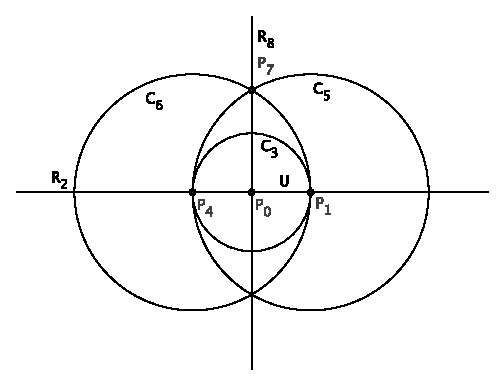
\includegraphics{1_Es1_perp}} 
%\includegraphics{Es1perpendicolare} 
\caption{Rette perpendicolari}
\end{center}
\end{figure}

%%%%%%%%%%%%%%%%%%%%%%%%%%%%%%%%%%%%%%% S1

\begin{align*}
S_{1} = ( &P_{0}, P_{1}, R_{2}(P_{0}, P_{1}), C_{3}(P_{0};\overline{P_{0} P_{1}}), \\
&P_{4}(C_{3}, R_{2} ), C_{5}(P_{1};\overline{P_{1} P_{4}}), C_{6}(P_{4};\overline{P_{1} P_{4}}),\\
&P_{7}(C_{5}, C_{6} ), R_{8}(P_{0}, P_{7}) )
\end{align*}




%%%
%%%%%%%%%%%%%%%%%%%%%%%%%% ESEMPIO ASSI CARTESIANI    %%%%%%%%%
\subsection{Sistema di assi cartesiani} \label{carte}
Per costruire un sistema di assi cartesiani, centrati in $P_{0}$ e di unità di misura $U$ data, si procede alla costruzione di due rette perpendicolari descritte dall'esempio precedente; dopodichè ciascuna retta può diventare asse del sistema cartesiano, con una ripartizione in segmenti di lunghezza $U$ attraverso la costruzione di circonferenze successive con centro nell'intersezione fra l'asse stesso e la circonferenza precedente. Si proceda nel seguente modo:

\begin{enumerate}

\item Si tracci la costruzione definita dalla successione $S_{1}$ dell'esempio precedente. 

\item Si rinominino i punti sugli assi, con una notazione più comoda: $P_{0} := P_{(0,0)}$ e $P_{1} := P_{(1,0)}$.

\item Si costruiscano le circonferenze $C_{(i,0)}(P_{(i,0)};\overline{U})$ sull'asse orizzontale di centro $P_{(i,0)}$ e di raggio $U$. Ciascuna di esse formerà due intersezioni, la prima nuova, che sarà chiamata $P_{(i+1,0)}$, e la seconda già costruita precedentemente e chiamata $P_{(i-1,0)}$, per $i = 1 ... n$

\item Si costruiscano con lo stesso procedimento del punto precedente, i punti $P_{(0,i)}$ che suddividono l'asse verticale in unità di misura di lunghezza $U$.

\end{enumerate}

\noindent
Le due rette perpendicolari $R_{2}(P_{0}, P_{1})$ e $R_{8}(P_{0}, P_{7})$ costruite formano gli assi cartesiani cercati. Le successioni di punti $P_{(i,0)}$ e $P_{(0,i)}$, suddividono gli assi nelle unità di misura del sistema.  
La costruzione euclidea appena descritta è data dalla successione:

%%%%%%%%%%%%%%%%%%%%%%%%%%%%%%%%%%%%%%% S 2

\begin{align*}
S_{2} = S_{1} \cup \{C_{(i,0)}(P_{(i,0)};\overline{U}), P_{(i+1,0)}, \mid  i \in (1,2\dots) \}  \\
 \{C_{(0,i)}(P_{(0,i)};\overline{U}), P_{(i+1,0)} \mid   i \in (1,2\dots) \} \cup \\
  \{C_{(i,0)}(P_{(i,0)};\overline{U}), P_{(i-1,0)}, \mid  i \in (-1,-2\dots) \}  \cup  \\
  \{C_{(0,i)}(P_{(0,i)};\overline{U}), P_{(i-1,0)} \mid  i \in (-1,-2\dots) \} 
\end{align*}


%%%%%%%%% IMMAGINE COSTRUZIONE ASSI % %%%%%%%%%%%%%%%%%%%%%

\begin{figure}[!h]
%centrare
\begin{center}
\resizebox{12.7 cm}{9.5 cm}{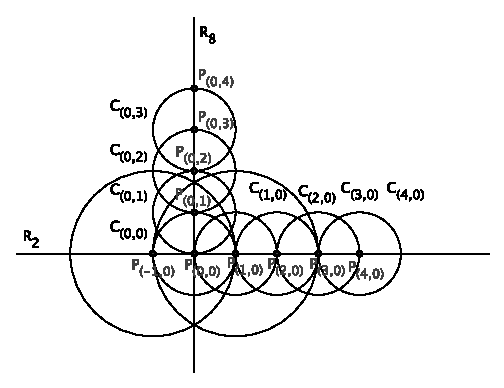
\includegraphics{1_Es_2_assi}} 
\caption{Assi cartesiani}
\end{center}
\end{figure}


%%%
%%%%%%%%%%%%%%%%%%%%%%%%%% Esempio BISETTRICE %%%%%%%%%%%%%
\subsection{Bisettrice di un quadrante} \label{bisett}
Per costruire la bisettrice dell'angolo formato fra due rette perpendicolari, si può procedere nel seguente modo:

\begin{enumerate}

\item Si tracci la successione definita dalla successione $S_{1}$ dell'esempio \ref{perp}.

\item Si evidenzi il punto $P_{9}(C_{3}, R_{8})$, come prima intersezione fra $C_{3}$ ed $R_{8}$.

\item Si tracci la circonferenza  $C_{10}(P_{9}; \overline{P_{1} P_{4}} )$.

\item Si evidenzi il punto $P_{11}(C_{5}, C_{10})$, come prima intersezione fra $C_{5}$ e $C_{10}$.

\item Si tracci infine la retta $R_{12}(P_{0}, P_{11} )$. 

\end{enumerate}

\noindent
La retta $R_{12}(P_{0}, P_{11} )$ è la bisettrice del primo e terzo quadrante cercata. La costruzione euclidea è data da:

%%%%%%%%%%%%%%%%%%%%%%%%%%%%%% S3 %%%%%%%%%%%
\begin{align*}
S_{3} = S_{1} \cup (P_{9}(C_{3}, R_{8}), C_{10}(P_{9}; \overline{P_{1}P_{4}} ),  \\
 P_{11}(C_{5}, C_{10}),  R_{12}(P_{0}, P_{11} ) ) \\
\end{align*}


%%%%%%%%% IMMAGINE COSTRUZIONE BISETTRICE ASSI %%%%%%%%%%%%%
\begin{figure}[!h]
%centrare
\begin{center}
\resizebox{12.7 cm}{9.5 cm}{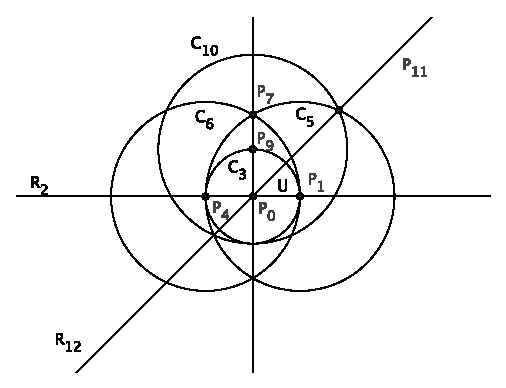
\includegraphics{1_Es3_bisett}} 
\caption{Bisettrice}
\end{center}
\end{figure}

%%%%%%%%%%%%%%%%%
%%%%%%%%%%%%%%%%%%%%%%%%%% Esempio PUNTO MEDIO%%%%%%%%%
\subsection{Punto medio} \label{medio}
Dato un segmento di estremi $P_{0}$ e $P_{1}$, procedendo nel seguente modo è possibile costruire il suo punto medio:

\begin{enumerate}

\item Si tracci il punto $P_{1}$ a distanza $U$ da $P_{0}$ in direzione arbitraria.

\item Si tracci la retta $R_{2}(P_{0}, P_{1})$.

\item Si tracci la circonferenza $C_{3}(P_{0}; \overline{P_{0} P_{1}})$.

\item Si tracci la circonferenza $C_{4}(P_{1}; \overline{P_{1} P_{0}})$.

\item Si evidenzi il primo punto di intersezione $P_{5}(C_{3},C_{4})$ fra le due circonferenze appena costruite, secondo l'ordine convenzionale.

\item Si evidenzi il secondo punto di intersezione  $P_{6}(C_{3},C_{4})$ fra le due circonferenze appena costruite, secondo l'ordine convenzionale.

\item Si tracci la retta $R_{7}(P_{5}, P_{6})$.

\item Si evidenzi il punto di intersezione $P_{8}(R_{2},R_{7})$.

\end{enumerate}

\noindent
Il punto  $P_{8}$ è il punto medio del segmento $ \overline{P_{0} P_{1}}$.
La costruzione euclidea è data da:

%%%%%%%%%%%%%%%%%%%%%%%%%%%%%% S4 %%%%%%%%%%%

\begin{align*}
S_{4} = (&P_{0}, P_{1}, R_{2}(P_{0}, P_{1}), C_{3}(P_{0}; \overline{P_{0} P_{1}}) \\
&C_{4}(P_{1}; \overline{P_{1} P_{0}}), P_{5}(C_{3},C_{4}), P_{6}(C_{4},C_{3}) \\
&R_{7}(P_{5}, P_{6}), P_{8}(R_{2},R_{7}) )
\end{align*}



%%%%%%%%% IMMAGINE COSTRUZIONE PUNTO MEDIO %%%%%%%%%%%%%

\begin{figure}[!h]
%centrare
\begin{center}
\resizebox{12.7 cm}{9.5 cm}{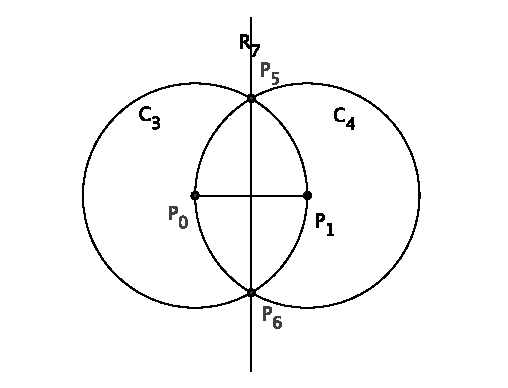
\includegraphics{1_Es4_puntomed}} 
\caption{Punto medio}
\end{center}
\end{figure} 


%%%%%%%%%
%%%%%%%%%%%%%%%%%%%%%%%%%% Esempio RETTA PARALLELA %%%%%%%%
\subsection{Retta parallela ad una retta data, per un punto dato} \label{parall}
Data una retta $R_{2}$ passante per $P_{0}$ e $P_{1}$, e un punto $P_{3}$ esterno alla retta, si richiede la costruzione con riga e compasso della parallela a $R_{2}$ passante per $P_{3}$. Per risolvere tale problema, si può applicare due volte la costruzione della perpendicolare ad una retta data, già proposto in \ref{perp}, nel seguente modo:

\begin{enumerate}

\item Si tracci il punto $P_{1}$ a distanza $U$ da $P_{0}$ in direzione arbitraria.

\item Si tracci la retta $R_{2}(P_{0}, P_{1})$, passante quindi per i punti $P_{0}$ e $P_{1}$.

\item Si evidenzi con $P_{3}$ il punto dato dal problema.

\item Si tracci la circonferenza $C_{4}(P_{3}; \overline{P_{3} P_{0}})$.

\item Si evidenzi $P_{5}(R_{2},C_{4})$, punto di intersezione fra $R_{2}$ e $C{4}$.

\item Si tracci la circonferenza $C_{6}(P_{0}; \overline{P_{0} P_{3}})$.

\item Si tracci la circonferenza $C_{7}(P_{5}; \overline{P_{5} P_{3}})$.

\item Si evidenzi $P_{8}(C_{6},C_{7})$, punto di intersezione fra $C_{6}$ e $C{7}$.

\item Si tracci la retta $R_{9}(P_{3}, P_{8})$. 

\item Si evidenzi $P_{10}(R_{2},R_{9})$, punto di intersezione fra $R_{2}$ e $R{9}$.

\item Si tracci $C_{11}(P_{3}; \overline{P_{3} P_{10}})$.

\item Si tracci il punto $P_{12}(R_{9}, C_{11})$.

\item Si tracci la circonferenza $C_{13}(P_{10}; \overline{P_{10} P_{12}})$.

\item Si tracci la circonferenza $C_{14}(P_{12}; \overline{P_{10} P_{12}})$

\item Si evidenzi $P_{15}(C_{13},C_{14})$, punto di intersezione fra $C_{13}$ e $C{14}$.

\item Si tracci la retta $R_{16}(P_{3}, P_{15})$. 

\end{enumerate}

\noindent 
La retta  $R_{16}(P_{3}, P_{15})$ è parallela alla retta data $R_{2}(P_{0}, P_{1})$ e passa per il punto dato $P_{3}$.
La costruzione euclidea appena descritta è data dalla successione: 

%%%%%%%%%%%%%%%%%%%%%%%%%%%%%%%%%%%%%%% S5

\begin{align*}
S_{5} = (&P_{0}, P_{1}, R_{2}(P_{0}, P_{1}), P_{3}, C_{4}(P_{3}; \overline{P_{3} P_{0}}) \\
&P_{5}(R_{2},C_{4}), C_{6}(P_{0}; \overline{P_{0} P_{3}}), C_{7}(P_{5}; \overline{P_{5} P_{3}}),  \\
&P_{8}(C_{6},C_{7}), R_{9}(P_{3}, P_{8}), P_{10}(R_{2},R_{9}), C_{11}(P_{3}; \overline{P_{3} P_{10}}) \\
&P_{12}(R_{9}, C_{11}), C_{13}(P_{10}; \overline{P_{10} P_{12}}) \\
&C_{14}(P_{12}; \overline{P_{10} P_{12}}), P_{15}(C_{13},C_{14}), R_{16}(P_{3}, P_{15}) )
\end{align*}

%%%%%%%% IMMAGINE COSTRUZIONE PARALLELE %
\begin{figure}[!h]
%centrare
\begin{center}
\resizebox{14.0 cm}{10.5 cm}{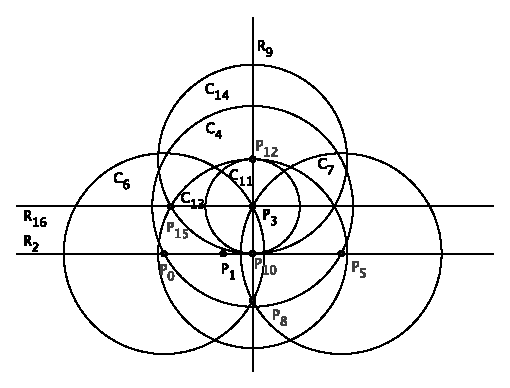
\includegraphics{1_Es5_parall}} 
%\includegraphics{Es1perpendicolare} 
\caption{Rette parallele}
\end{center}
\end{figure}


%%%
%%%%%%%%%%%%%%%%%%% ESEMPIO 2 SEGMENTI  %%%%%%%%%%%%%%%%

\subsection{Manipolazione di due segmenti}  \label{segm}

Questo particolare problema prevede, oltre all'uso di riga non graduata e di compasso, anche l'uso di due segmenti di lunghezza data. Dati quindi due segmenti $\alpha$ e $\beta$ $(\alpha > \beta)$, saranno proposte le costruzioni dei segmenti di lunghezza $\alpha + \beta$, $\alpha - \beta$, $\alpha \cdot \beta$ e $\alpha/\beta$. Inoltre verrà proposta la costruzione di $\alpha^{-1}$. Tali possibilità danno al procedimento di costruzione con riga e compasso la struttura di campo. 


%%%%%%%%%%%%%%%%%%%%%%%%%%%%%%%%%%%%%%%%%%%%%%%%%%%%%%%%%
%%% SOMMA E DIFFERENZA
\subsubsection{Somma e differenza dei segmenti dati}
Si propone il procedimento per la costruzione di $\alpha + \beta$ e $\alpha - \beta$:
\begin{enumerate}

\item Si pongano su una linea retta $R$ i segmenti dati $\alpha$ e $\beta$, in questo ordine, con un solo punto di intersezione.

\item Si evidenzi con  $P_{0}$ e  $P_{1}$ gli estremi di $\alpha$; con $P_{1}$ e $P_{2}$ gli estremi di $\beta$.

\item Si tracci la circonferenza $C_{3}(P_{1}; \overline{P_{1} P_{2}})$.

\item Si evidenzi con $P_{4}(C_{3},R)$,  l'intersezione non ancora tracciata fra la circonferenza e la retta.

\end{enumerate}

A questo punto si ha il segmento $P_{0} P_{2}$, di lunghezza $\alpha + \beta$, e il segmento $P_{0} P_{4}$ di lunghezza $\alpha - \beta$ \\ \\


%%%%%%%%% PRIMA e seconda IMMAGINE COSTRUZIONE 2 segmenti! %
\begin{figure}%
\begin{center}%
\subfigure[$\alpha + \beta$, $\alpha - \beta$]{
\resizebox{6.0 cm}{4.5 cm}{\includegraphics{1_Es6_1a}} 
}
\hspace{.20in}%
\subfigure[$\alpha \cdot \beta$]{
\resizebox{5.5 cm}{4.0 cm}{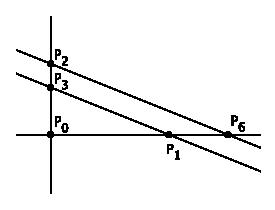
\includegraphics{1_Es6_1b}} 
}
\end{center}%
\caption{Manipolazione di segmenti 1}%
\end{figure}


%%%%%%%%%%%%%%%%%%%%%%%%%%%%%%%%%%%%%%%%%%%%%%%%%%%%%%%%%%%%% PRODOTTO
\subsubsection{Prodotto dei segmenti dati}
Si propone il procedimento per la costruzione di $\alpha \cdot \beta$:

\begin{enumerate}

\item Dopo aver costruito due rette perpendicolari centrate in $P_{0}$, si pone sull'asse orizzontale il segmento $\alpha$, con estremi $P_{0} P_{1}$ e sull'asse verticale il segmento $\beta$, con estremi $P_{0} P_{2}$.

\item Si tracci il punto $P_{3}$ a distanza $U$ da $P_{0}$, sull'asse verticale.

\item Si tracci la retta $R_{4}(P_{1}, P_{3})$.

\item Si tracci la retta $R_{5}$ parallela ad $R_{4}$ e passante per $P_{2}$, usando il procedimento dell'esempio precedente.

\item Si evidenzi il punto $P_{6}$ di intersezione fra $R_{5}$ e l'asse orizzontale. 

\end{enumerate}

Da questa costruzione, applicando il teorema di Talete, si può affermare che

\begin{align*}
\frac{P_{0}P_{6}}{\alpha} = \frac{\beta}{U}
\end{align*}

Dato che U è unità di misura iniziale, si può porre arbitrariamente uguale ad $1$, per ottenere

\begin{align*}
\frac{P_{0}P_{6}}{\alpha} = \beta
\end{align*}

Da cui si deduce che il segmento $P_{0}P_{6}$, è il segmento di lunghezza $\alpha \cdot \beta$ cercato. \\ 


%%%%%%%%%%%%%%%%%%%%%%%%%%%%%%%%%%%%%%%%%%%%%%%%%%%%%%%%%%%%% RAPPORTO
\subsubsection{Rapporto dei segmenti dati}
Si propone il procedimento per la costruzione di $\alpha/\beta$:

\begin{enumerate}

\item Dopo aver costruito due rette perpendicolari centrate in $P_{0}$, si pone sull'asse orizzontale il segmento $\alpha$, con estremi $P_{0} P_{1}$ e sull'asse verticale il segmento $\beta$, con estremi $P_{0} P_{2}$.

\item Si tracci il punto $P_{3}$ a distanza $U$ da $P_{0}$, sull'asse verticale.

\item Si tracci la retta $R_{4}(P_{1}, P_{2})$, che congiunge gli estremi di $\alpha$ e $\beta$.

\item Si tracci la retta $R_{5}$ parallele a $R_{4}$ passante per $P_{3}$, usando il procedimento dell'esempio \ref{parall}.

\item Si evidenzi il punto $P_{6}$ di intersezione fra $R_{5}$ e l'asse orizzontale.

\end{enumerate}

Nella costruzione appena descritta vale la seguente proporzione:

\begin{align*}
\frac{P_{0}P_{6}}{U} = \frac{\alpha}{\beta}
\end{align*}

dalla quale, ponendo U = 1, si ottiene

\begin{align*}
P_{0}P_{6} = \frac{\alpha}{\beta}
\end{align*}

Quindi il segmento $P_{0}P_{6}$, è il segmento di lunghezza $\alpha / \beta$ cercato. \\ 

%%%%%%%% Terza e quarta IMMAGINE COSTRUZIONE 2 segmenti! %
\begin{figure}%
\begin{center}%
\subfigure[$\alpha / \beta$]{
\resizebox{6.0 cm}{4.5 cm}{\includegraphics{1_Es6_2a}} 
}
%\hspace{.25in}%
\subfigure[$\alpha^{-1}$]{
\resizebox{6.0 cm}{4.5 cm}{\includegraphics{1_Es6_2b}} 
}
\end{center}%
\caption{Manipolazione di segmenti 2}%
\end{figure}

%%%%%%%%%%%%%%%%%%%%%%%%%%%%%%%%%%%%%%%%%%%%%%%%%%%%%%%%%%%%%% INVERSO
\subsubsection{Inverso del segmento dato}
Si propone, per ultimo, il procedimento per la costruzione di $\alpha^{-1}$.
\begin{enumerate}
\item Dopo aver costruito due rette perpendicolari centrate in $P_{0}$, si pone sull'asse orizzontale il segmento $\alpha$, con estremi $P_{0} P_{1}$.

\item Si tracci il punto $P_{2}$ a distanza $U$ da $P_{0}$, sull'asse orizzontale.

\item Si tracci il punto $P_{3}$ a distanza $U$ da $P_{0}$, sull'asse verticale.

\item Si tracci la retta $R_{4}(P_{1}, P_{3})$, che congiunge gli estremi di $\alpha$ a quelli del segmento unitario verticale.

\item Si tracci la retta $R_{5}$, parallele a $R_{4}$ passante per $P_{2}$, usando il procedimento dell'esempio \ref{parall}.

\item Si evidenzi il punto $P_{6}$ di intersezione fra $R_{5}$ e l'asse verticale.
\end{enumerate}

Nella costruzione appena descritta, vale la seguente proporzione:

\begin{align*}
 \frac{U}{\alpha} = \frac{P_{0}P_{6}}{U}
\end{align*}

dalla quale, ponendo U = 1, si ottiene 

\begin{align*}
P_{0}P_{6} = \alpha^{-1}
\end{align*}

Quindi $P_{0}P_{6}$ è  il segmento di lunghezza $\alpha^{-1}$ cercato. 


%%%%%%%%%%%%%%%%%%% ESEMPIO RADICE
%%
\subsection{Radice quadrata di un segmento dato} \label{radi}

Posto $U = 1$, si vuole costruire un segmento di lunghezza $\sqrt{\alpha}$, dove $\alpha$ è un segmento di lunghezza nota. Si propone la seguente costruzione:

\begin{enumerate}

\item Si tracci il punto $P_{1}$ a distanza $1$ da $P_{0}$ in direzione arbitraria.

\item Si costruiscano i due assi cartesiani ortogonali centrati su $P_0$ con ascisse in direzione $P_1$, utilizzando il procedimento visto in \ref{perp} ed ottenendo quindi la costruzione iniziale
\begin{align*}
S_{1} = ( &P_{0}, P_{1}, R_{2}(P_{0}, P_{1}), C_{3}(P_{0};\overline{P_{0} P_{1}}), \\
&P_{4}(C_{3}, R_{2} ), C_{5}(P_{1};\overline{P_{1} P_{4}}), C_{6}(P_{4};\overline{P_{1} P_{4}}),\\
&P_{7}(C_{5}, C_{6} ), R_{8}(P_{0}, P_{7}) )
\end{align*}
\noindent
Nella figura proposta compariranno per chiarezza solo gli elementi essenziali $P_0, P_1, R_2, P_4, R_8$.

\item Si disegni la circonferenza $C_{9}(P_{0}; \alpha )$  di centro $P_0$ e raggio $\alpha$.

\item Si evidenzi il punto $P_{10}(C_{9}, R_{2} )$, quindi come intersezione fra $C_{3}$ e $R_{2}$. E' stato così ottenuto il segmento $\overline{P_{4}P_{10}}$ di lunghezza $\alpha + 1$.

\item Si trovi il punto medio di $\overline{P_{4} P_{10}}$, dato da $P_{16}$, trovato con il seguente procedimento: 
\begin{align*}
S'_{4} = ( &C_{11}(P_{4}, \overline{P_{4} P_{10}}) ), C_{12}(P_{10}, \overline{P_{10} P_{4}}), \\
&P_{13}(C_{11},C_{12}), P_{14}(C_{11},C_{12}), \\ 
&R_{15}(P_{13}, P_{14}), P_{16}(R_{2},R_{15}) )
\end{align*}
\noindent
analogo a quello usato in \ref{medio}. Nella figura, comparirà per chiarezza solo il punto medio risultante del procedimento e la retta $R_{15}$ passante per esso e perpendicolare a $P_2$.

\item Si tracci la circonferenza $C_{17}(P_{16};\overline{P_{16}P_{10}})$, avente quindi come diametro il segmento $\overline{P_{4}P_{10}}$.

\item Si evidenzi il punto $P_{18}(C_{17}, R_{8} )$.
\end{enumerate}

%%%%%%%% IMMAGINE COSTRUZIONE RADICE QUADRATA %
\begin{figure}[!h]
%centrare
\begin{center}
\resizebox{12.7 cm}{9.5 cm}{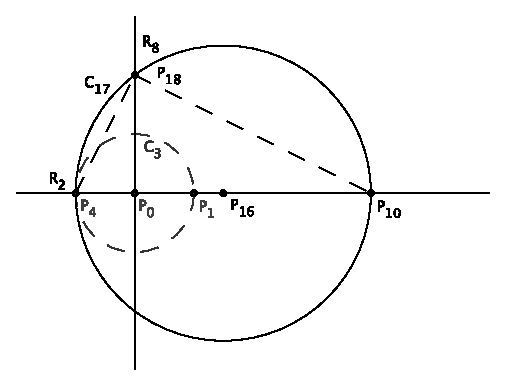
\includegraphics{1_Es7_radice}} 
%\includegraphics{Es1perpendicolare} 
\caption{Radice quadrata di $\alpha$}
\end{center}
\end{figure}

%%%%%%%%%%%%%%%%%%%%%%%%%%%%%%%%%%%%%%% S6

\noindent 
Nella costruzione ottenuta, dato che i triangoli $ P_{4}P_{0} P_{18}$ e $P_{0} P_{18} P_{10}$ sono simili, sussiste la seguente proporzione:
\begin{align*}
P_{4} P_{0} : P_{0} P_{18} = P_{0}P_{18} :P_{0}P_{10}
\end{align*}
Cioè
\begin{align*}
1 : P_{0}P_{18} = P_{0}P_{18} : \alpha
\end{align*}
Da cui si ricava che 
\begin{align*}
P_{0} P_{18} = \sqrt{ \alpha}
\end{align*}
Da questa osservazione si deduce un importante risultato: per ogni segmento dato, di lunghezza $\alpha$, è sempre possibile costruire il segmento di lunghezza $\sqrt{ \alpha}$. 

La costruzione euclidea del procedimento appena descritto è data da:
\begin{align*}
S_{6} = ( &P_{0}, P_{1}, R_{2}(P_{0}, P_{1}), C_{3}(P_{0};\overline{P_{0} P_{1}}), \\
&P_{4}(C_{3}, R_{2} ), C_{5}(P_{1};\overline{P_{1} P_{4}}), C_{6}(P_{4};\overline{P_{1} P_{4}}),\\
&P_{7}(C_{5}, C_{6} ), R_{8}(P_{0}, P_{7}), C_{9}(P_{0}; \alpha ), P_{10}(C_{9}, R_{2} ) \\
&C_{11}(P_{4}, \overline{P_{4} P_{10}}) ), C_{12}(P_{10}, \overline{P_{10} P_{4}}), \\
&P_{13}(C_{11},C_{12}), P_{14}(C_{11},C_{12}),   R_{15}(P_{13}, P_{14}), \\
&P_{16}(R_{2},R_{15}) ), C_{17}(P_{16};\overline{P_{16} P_{10}}), P_{18}(C_{17}, R_{8} ) )
\end{align*}


%FINE CAPITOLO 1
%LABELS

%\label{perp}
%\label{carte}
%\label{bisett}
%\label{medio}
%\label{parall}
%\label{segm}
%\label{radi}



%%%%%%%%%%%%%%%%%%%%%%%%%%%%%%%%%%%%%%%%%%%%
%CAPITOLO NUMERI EUCLIDEI
%%%%%%%%%%%%%%%%%%%%%%%%%%%%%%%%%%%%%%%%%%%%

\chapter{Numeri euclidei}

%%%%%%%%%%%%%%%%%%%%%%%%%% SEZIONE %%%%%%%%%%%%
\section{Costruzioni euclidee nel piano reale}
Ora che si ha una definizione formale delle costruzioni euclidee, intese come successioni di punti, rette e circonferenze fra loro correlate, è necessario esprimere la loro interazione con i punti del piano reale e quindi le proporietà, in termini algebrici, di questa struttura.

%%% Def della funzione principale
\begin{definizione} \label{immers}
L'insieme delle possibili costruzioni euclidee, aventi $P_0$ e $P_1$ come punti iniziali, indicato con $\mathcal{E}(P_0,P_1)$, può essere immerso nel piano $\mathbb{R}\times\mathbb{R}$, definendo la seguente funzione:
\begin{align*} 
\mathcal{I}:  \mathcal{E}(P_0,P_1) & \longrightarrow \mathbb{R}\times\mathbb{R} 
\end{align*}
%itemize della definizione
\begin{enumerate}

\item Se $K_{i} \in \mathcal{E}(P_0,P_1) $ è uno dei due punti iniziali $P_0$ o $P_1$, allora 
\begin{align*} 
\mathcal{I}:  \mathcal{E}(P_0,P_1) & \longrightarrow \mathbb{R}\times\mathbb{R} \\
P_0 & \longmapsto (0,0) \\
P_1 & \longmapsto (1,0) \\
\end{align*}

\item Se $K_{i} \in \mathcal{E}(P_0,P_1)$ è una retta fra due punti $K_{m}$ e $K_{n}$, allora 
\begin{align*} 
\mathcal{I}:  \mathcal{E}(P_0,P_1) & \longrightarrow \mathbb{R}\times\mathbb{R} \\
K_{i}  & \longmapsto R_{i} (  \mathcal{I} (K_{m}), \mathcal{I}(K_{n}) ) 
\end{align*}
Quindi la retta per i due punti $K_{m}, K_{n}$ di $\mathcal{E}(P_0,P_1)$ viene mappata da $ \mathcal{I}$ nella retta su $\mathbb{R}\times\mathbb{R}$ passante per le immagini dei medesimi punti $K_{m}, K_{n} $, cioè $ \mathcal{I} (K_{m}), \mathcal{I}(K_{n}) $.

\item Se $K_{i} \in \mathcal{E}(P_0,P_1)$ è una circonferenza di centro $K_{c}$ e di raggio il segmento avente per estremi i punti $K_{r}$ e $K_{s}$, allora 
\begin{align*} 
\mathcal{I}:  \mathcal{E}(P_0,P_1) & \longrightarrow \mathbb{R}\times\mathbb{R} \\
K_{i}  & \longmapsto C_{i} (  \mathcal{I} (K_{c}); \overline{  \mathcal{I}(K_{r}) \mathcal{I}(K_{s})})
\end{align*}

\item Se $K_{i} \in \mathcal{E}(P_0,P_1)$ è un punto di intersezione fra due circonferenze $C_{a}$, $C_{b}$, oppure di due rette $R_{a}$, $R_{b}$, oppure di una retta $R_{a}$ e una circonferenza $C_{b}$, allora si ha rispettivamente
\begin{align*} 
\mathcal{I}:  \mathcal{E}(P_0,P_1) & \longrightarrow \mathbb{R}\times\mathbb{R} \\
K_{i}  & \longmapsto P_{i} ( \mathcal{I}(C_{a}),   \mathcal{I}(C_{b})) \\
K_{i}  & \longmapsto P_{i} ( \mathcal{I}(R_{a}),   \mathcal{I}(R_{b})) \\
K_{i}  & \longmapsto P_{i} ( \mathcal{I}(R_{a}),   \mathcal{I}(C_{b})) 
\end{align*}
\end{enumerate}

Si ottiene quindi l'insieme delle costruzioni euclidee con unità di misura iniziale pari a $1$ immersa nel piano reale. I suoi elementi saranno chiamati \begin{bfseries}costruzioni euclidee nel piano reale\end{bfseries} e saranno indicati con $\mathcal{E}_{\mathbb{R}\times\mathbb{R}}$. 
\end{definizione} 

%%%%% Osservazio sulla biezione
\begin{osservazione}
La definizione precedente garantisce l'esistenza di una biiezione fra i punti, le rette e le circonferenze  delle costruzioni euclidee, con quelle disegnate sul piano reale.
\begin{align*}
\mathcal{I}:  \mathcal{E}(P_0,P_1) & \longrightarrow   \mathcal{E}_{\mathbb{R}\times\mathbb{R}} \subset \mathbb{R}\times\mathbb{R} 
\end{align*}
Ad ogni punto delle costruzioni euclidee corrisponde quindi un solo punto delle costruzioni euclidee nel piano reale.
\end{osservazione}

%% def di punti euclidei
\begin{definizione}
Un punto $Q$ di $\mathbb{R}\times\mathbb{R}$ che compare in una costruzione euclidea nel piano, cioè tale che $Q \in \mathcal{E}_{\mathbb{R}\times\mathbb{R}}$ è detto \begin{bfseries}punto euclideo\end{bfseries}  o costruibile. L'insieme di tutti i punti euclidei sarà indicato con $\mathfrak{E}$.
\end{definizione}

\begin{osservazione} \label{osservaz}
L'insieme di punti $\mathbb{Z}\times \mathbb{Z} := \{(m,n) \mid m \in \mathbb{Z}, n \in \mathbb{Z}\}$ è un sottoinsieme di $\mathfrak{E}$, infatti, come visto in \ref{carte}, a partire dai punti iniziali $P_0$ e $P_1$ è possibile costruire un sistema di assi cartesiani ortogonali, i cui punti vanno a ricalcare $\mathbb{Z}\times \mathbb{Z}$ nelle costruzioni euclidee nel piano reale.
\end{osservazione}

Si presentano ancora le definizioni di numero reale euclideo e numero complesso euclideo, strettamente correlate con la definizione di punto euclideo:

%%%%%%%%%%%%%% Numero reale Euclideo
\begin{definizione}
$\gamma \in \mathbb{R}$ è detto \begin{bfseries}numero reale euclideo\end{bfseries} se esiste una costruzione euclidea nel piano reale nella quale compare un segmento di lunghezza $|\gamma|$.
\end{definizione}

%%%%%%%%%%% Numero complesso  Euclideo
\begin{definizione}
$a + i b \in \mathbb{C}$ è detto \begin{bfseries}numero complesso euclideo\end{bfseries} se il corrispondente punto $(a, b) \in \mathbb{R}\times\mathbb{R}$ appartiene ad una costruzione euclidea nel piano reale.
\end{definizione}

%%%%%%%%%%%%% Osservazione reali-complessi
\begin{osservazione}
Si osserva che un punto è euclideo se e solo se lo sono le sue rispettive coordinate nel piano reale. Infatti dato $P$ euclideo nel piano reale, è sempre possibile tracciare le rette parallele agli assi (\ref{parall}), e passanti per $P(a, b)$. Queste rette tagliano sugli assi due segmenti di lunghezza $|a|$ e $|b|$, quindi $a$ e $b$ sono numeri reali euclidei. Viceversa se $a$ e $b$ sono due numeri euclidei, allora posso sempre costruire i segmenti di lunghezza $|a|$ e $|b|$. Una volta tracciati, rispettivamente sull'asse $x$ e sull' asse $y$, si ottengono i numeri complessi euclidei $a$ ed $ ib$. Tracciando le rette parallele agli assi, e passanti per $a$ e $ ib$ si ottiene il punto di intersezione $P(a,b)$, che è quindi costruibile. 
Questo significa che si può parlare in modo equivalente di punti euclidei e numeri reali euclidei sul piano reale.
\end{osservazione}

%%%%%%%%%%%%%%%%%%%%%%%%%%%%%%%%%%%%%%%%%%%%%%%%
%%%%%%%%%%%%%%%%%%%%%%% SEZIONE %%%%%%%%%%%%%%%%%%%%
\section{Caratterizzazione di $\mathfrak{E}$} 
Lo scopo del paragrafo precedente è stato la definizione di $\mathfrak{E}$; in questo verranno analizzate le sue proprietà, tratte da \cite{cattaneo} e \cite{Procesi}, e ne verrà data una caratterizzazione algebrica.

% proprietà di caratterizzazione di E come campo
\begin{prop} \label{propcaratt}
Dato $\mathfrak{E}$, insieme dei punti euclidei del piano reale, si ha che
\begin{enumerate} [i)]
\item $\mathbb{Z} \subset \mathfrak{E}$ 
\item $\mathbb{Q} \subset \mathfrak{E}$
\item $\mathfrak{E}$ è un campo.
\end{enumerate}
\end{prop}

\begin{proof}
\begin {enumerate} [i)]
\item Segue da \ref{osservaz}.
\item E' sufficiente provare che ogni numero della forma $1/n$ è costruibile. Segue da \ref{segm}.
\item Per provare che $\mathfrak{E}$ è un campo, si deve dimostrare che vale l'implicazione
\begin{equation}
\forall \alpha, \beta \in\mathfrak{E} \Rightarrow \alpha \pm \beta \in \mathfrak{E}  \wedge  \alpha\beta\in \mathfrak{E}  \wedge \alpha / \beta \in \mathfrak{E}
\end{equation}
Segue da \ref{segm}. 
\end{enumerate}
\end{proof}

%osservazione su E come estensione di grado due
\begin{osservazione} \label{osscaratt}
Da \ref{radi} si ha la seguente importante proposizione per le costruzioni euclidee: se un numero $z$ è costruibile allora lo è anche la sua radice quadrata.
\begin{align*}
\forall z \in \mathfrak{E} \Rightarrow \sqrt{z} \in \mathfrak{E}
\end{align*}
\end{osservazione}

%%%%%%%%%%%% primo ragionamento
\noindent
Per l'osservazione \ref{osscaratt}, e per la proprietà \ref{propcaratt} si può affermare che:
\begin{align*}
\forall q_0 \in \mathbb{Q} \Rightarrow \sqrt{q_0} \in \mathfrak{E}
\end{align*}
\noindent
Quindi
\begin{align*}
\mathbb{Q} \subset \mathbb{Q}(\sqrt{q_0}) \subset \mathfrak{E}
\end{align*}
\noindent
dove $\mathbb{Q}(\sqrt{q_0})$ è il più piccolo campo che estende $\mathbb{Q}$ contenente $\sqrt{q_0}$.

%%%%%%%%%%%%% secondo ragionamento
\noindent
Ripetendo il ragionamento precedente, si ha che
\begin{align*}
\forall q_1 \in \mathbb{Q}(\sqrt{q_0}) \Rightarrow q_1 \in \mathfrak{E} \Rightarrow \sqrt{q_1} \in \mathfrak{E}
\end{align*}
\noindent
Quindi si può affermare che: 
\begin{align*}
\mathbb{Q}\subset \mathbb{Q}(\sqrt{q_0}) \subset  \mathbb{Q}(\sqrt{q_0},\sqrt{q_1}) \subset \mathfrak{E}
\end{align*}
\noindent
%%%%%%%%%%% terzo ragionamento
Ripetendo ancora il ragionamento, si ha che
\begin{align*}
\forall q_2 \in \mathbb{Q}(\sqrt{q_0},\sqrt{q_1})  \Rightarrow q_2 \in \mathfrak{E} \Rightarrow \sqrt{q_2} \in \mathfrak{E}
\end{align*}

\noindent
Quindi si può affermare che 
\begin{align*}
\mathbb{Q}\subset \mathbb{Q}(\sqrt{q_0}) \subset  \mathbb{Q}(\sqrt{q_0},\sqrt{q_1}) \subset \mathbb{Q}(\sqrt{q_0},\sqrt{q_1}, \sqrt{q_2}) \subset \mathfrak{E}
\end{align*}
\noindent
In questo modo si può continuare ad estendere il campo $\mathbb{Q}$ indefinitamente, ottenendo sempre un sottocampo di $\mathfrak{E}$.
%%%%%%%%%%%% finale de ragionamento
\\

L'idea appena presentata serve a caratterizzare ulteriormente $\mathfrak{E}$, come una successione di estensioni di campi. Inoltre esso fornisce delle informazioni di fondamentale importanza sul grado di queste estensioni; infatti $[ \mathbb{Q}(\sqrt{q_0}), \mathbb{Q}] \leq 2$ e  $ [ \mathbb{Q}(\sqrt{q_0},\sqrt{q_1}), \mathbb{Q}(\sqrt{q_0})] \leq 2  $.
%%%%%%%%%%% intro al teorema  con FOOTNOTE!!!! %%%%%%%%%%%
\\ \\
Il prossimo teorema\footnote{Presentato in: \cite{cattaneo} Proposizione $7.1.10$ di  pag. 345,  \cite{Procesi} Teorema $7.4$ di pag. $23$, \cite{Artin} Teorema $4.9$  pag. 504. Si segue la dimostrazione di \cite{Procesi}. }, enuncia in modo formale quanto detto fino ad ora. 

%%%%%%%%%  teorema fondamentale
\begin{teorema} \label{tfond}
Un numero complesso $\alpha$ è euclideo se e solo se esiste una successione di campi 
\begin{align*}
\mathbb{Q} = \mathbb{E}_0 \subseteq \mathbb{E}_1 \subseteq ... \subseteq  \mathbb{E}_{n+1}  
\end{align*}
\noindent
che soddisfi le due condizioni seguenti:
\begin{enumerate}
\item $\alpha \in  \mathbb{E}_{n+1}$
\item $[\mathbb{E}_{j+1}, \mathbb{E}_{j}] \leq 2 \qquad j = 0, 1, ... , n $
\end{enumerate}
\end{teorema}

%%%%%%%%%%%%%%%%%%%%%%%%%%%%%
%%%%%%%%%%%%%%%inizio dimostrazione RIGHT
\begin{proof}
$\Rightarrow)$ Per ipotesi $\alpha = a+ ib$ è euclideo, quindi esiste una costruzione euclidea in cui compare il punto $P = (a,b)$, indicata con $(K_0, K_1, ..., K_n = P)$. 

%%%%%%%% Enumerazione 1
\begin{enumerate}

\item Si costruisce per induzione una successione di campi $\mathbb{Q} = \mathbb{E}_0 \subseteq \mathbb{E}_1 \subseteq ... \subseteq  \mathbb{E}_{n+1}$ che soddisfa la condizione $1$. Sia quindi $\mathbb{E}_j$ campo già costruito che verifica la condizione $1$, allora il successivo $\mathbb{E}_{j+1}$ lo si costruisce nel seguente modo: si considera il corrispondente elemento $K_{j+1}$ della costruzione euclidea.

%%%%%%%%% inizio Itemize 1.1
\begin{itemize}

\item Se $K_{j+1}$ è una retta o una circonferenza, si pone $\mathbb{E}_{j+1}=\mathbb{E}_{j}$

\item Se $K_{j+1}$ è un punto di coordinate $(c,d)$, si pone  $\mathbb{E}_{j+1}=\mathbb{E}_{j}(c,d)$, cioè l'estensione di $\mathbb{E}_{j}$ con i reali $(c,d)$.

\item Quando si è arrivati al penultimo campo, cioè $\mathbb{E}_{n}$, lo si estende con $\mathbb{E}_{n+1}=\mathbb{E}_{n}(i)$, dove i è l'unità immaginaria. Infatti, dato che $K_n = P = (a,b)$, e per il fatto che $i \in \mathbb{E}_{n+1}=\mathbb{E}_{n}(i) = \mathbb{E}_{n-1}(a,b)(i)$, si ha che $\alpha \in \mathbb{E}_{n+1}$.

\end{itemize}
%%%%%%%%%%%%% fine itemize 1.1

Prima di affrontare la dimostrazione del punto $2$ si prova che, se $K_{j}$ è una retta o una circonferenza allora la sua equazione cartesiana può essere scelta a coefficienti in $\mathbb{E}_k$

%%%%%%%%%%%%% inizio Itemize 1.2
\begin{itemize}

\item Se $K_{j}$ è una retta, allora passa per due punti della successione dati da $K_{s}$,  $K_{t}$ con $s,t \leq k$. La formula della retta per due punti, nota dalla geometria analitica, si basa sulle coordinate di $K_{s}$ e $K_{t}$, che sono rispettivamente nei campi $\mathbb{E}_s$, $\mathbb{E}_t$ e quindi nel campo $\mathbb{E}_j$.

\item Se $K_{j}$ è una circonferenza, analogamente, il centro e gli estremi del segmento di lunghezza del raggio sono dati da $K_{s}$, $K_{t}$ e $K_{u}$, con $s,t,u \leq k$. La formula della circonferenza ha come coefficienti elementi nei rispettivi campi $\mathbb{E}_s$, $\mathbb{E}_t$, $\mathbb{E}_u$ e quindi nel campo $\mathbb{E}_j$.

\end{itemize}
%%%%%%%%%%%%% fine itemize 1.2

%%% dim punto 2)
\item Si costruisce per induzione una successione di campi $\mathbb{Q} = \mathbb{E}_0 \subseteq \mathbb{E}_1 \subseteq ... \subseteq  \mathbb{E}_{n+1}$ che soddisfa la condizione $2$. Si dimostra che  $[\mathbb{E}_{j+1}, \mathbb{E}_{j}] \leq 2 $ per $j = 0, 1, ... , n$.
Si distinguono i seguenti tre casi:

%%%%%%%%%%%%% inizio Itemize 1.3
\begin{itemize}

\item Se $K_{j}$ è una retta o una circonferenza, si ha dal punto precedente che $\mathbb{E}_{j}=\mathbb{E}_{j-1}$ da cui segue $[\mathbb{E}_{j}, \mathbb{E}_{j-1}] = 2$.

\item Se $K_{j}$ è un punto allora può essere intersezione di due rette, di una retta e una circonferenza o di due circonferenza o di due circonferenze; si distinguono quindi i seguenti sottocasi:

%%%%%%%%%%%%%%%%%%%%% inizio enumerate 1.2.1
\begin{enumerate} [i)]

 \item  $K_{j}$ è intersezione di due rette, $K_{s}$, $K_{t}$ con $s,t \leq j$ allora, per quanto visto prima, si ha che le equazioni cartesiane delle due rette $K_{s}$ e $K_{t}$ sono a coefficienti in $\mathbb{E}_{j}$. Quindi le coordinate di $K_{j}$, ottenute risolvendo il sistema fra le due rette, sono in $\mathbb{E}_{j}$. Si ha che $[\mathbb{E}_{j}, \mathbb{E}_{j-1}] = 1$.

\item  $K_{j}$ è intersezione di una retta $K_{s}$ e una circonferenza, $K_{t}$ con $s,t \leq j$, le sue coordinate sono la soluzione del sistema:

\begin{displaymath}
 \left\{ \begin{array}{ll}
 K_{s}: ax + by + c = 0                             &     a,b,c \in \mathbb{E}_{j-1} \\
 K_{t}: x^2 + y^2 +dx + ey + f = 0           &     d,e,f \in \mathbb{E}_{j-1}
 \end{array} \right.
 \end{displaymath}
 
Per quanto visto prima i coefficienti $a,b,c,d,e,f$  sono tutti in $\mathbb{E}_{j}$. Se per esempio $a \neq 0$ (o analogamente $b \neq 0$), per sostituzione si ottiene il sistema :

\begin{displaymath}
 \left\{ \begin{array}{ll}
 x = -(b/a)y - (c/a)                          &     a,b,c \in \mathbb{E}_{j-1} \quad a \neq 0 \\
 y^2 + ly + m = 0                           &     l,m \in \mathbb{E}_{j-1}
 \end{array} \right.
 \end{displaymath}
 
L'equazione $y^2 + ly + m = 0$ può essere risolubile in $\mathbb{E}_{j-1}$ o meno. Si distinguono allora gli ulteriori due sottocasi:

%%%%%%%%%%%%%%%%%%% Inizio itemize 1.2.1.1
\begin{itemize}
 
 \item Se $y^2 + ly + m = 0$ è risolubile in $\mathbb{E}_{j-1}$ (quindi il corrispondente polinomio è riducibile in $\mathbb{E}_{j}$ ), allora si ha che $\mathbb{E}_{j} = \mathbb{E}_{j-1}$. Cioè $[\mathbb{E}_{j}, \mathbb{E}_{j-1}] = 1$.
 
 \item Se $y^2 + ly + m = 0$ non è risolubile in $\mathbb{E}_{j-1}$ (quindi il corrispondente polinomio, essendo di secondo grado, non è riducibile in $\mathbb{E}_{j-1}$ ), allora la soluzione del sistema estenderà il campo $\mathbb{E}_{j-1}$ con il campo $\mathbb{E}_{j}$ contenente le radici
 
\begin{displaymath}
\left\{ \begin{array}{ll}
y_1 = -l -\sqrt{l^2 - 4m}                        &     l,m \in \mathbb{E}_{j-1}  \\
y_2 = -l +\sqrt{l^2 - 4m}                     &     l,m \in \mathbb{E}_{j-1}
\end{array} \right.
\end{displaymath}

Cioè $\mathbb{E}_{j}  =  \mathbb{E}_{j-1} (\sqrt{l^2 - 4m}))$. Ma questo implica $[\mathbb{E}_{j}, \mathbb{E}_{j-1}] = 2$.
 
\end{itemize}
 
\item  $K_{j}$ è intersezione di due circonferenze $K_{s}$,  $K_{t}$ con $s,t \leq k$. Il ragionamento è analogo al precedente, si ha infatti il sistema:

\begin{displaymath}
 \left\{ \begin{array}{ll}
 K_{s}: x^2 + y^2 + ax + by + c = 0         &     a,b,c \in \mathbb{E}_{j-1} \\
 K_{t}: x^2 + y^2 +dx + ey + f = 0           &     d,e,f \in \mathbb{E}_{j-1}
 \end{array} \right.
 \end{displaymath}

Che equivale a 
\begin{displaymath}
 \left\{ \begin{array}{ll}
 K_{s}: x^2 + y^2 + ax + by + c = 0         &     a,b,c \in \mathbb{E}_{j-1} \\
 K_{t}: (a-d)x + (b-e)y + (c-f) = 0           &     d,e,f \in \mathbb{E}_{j-1}
 \end{array} \right.
 \end{displaymath}
 
 Riconducibile direttamente al caso precedente.
\end{enumerate}
%%%%%%%%%%%%%%%%%%%%% fine enumerate 1.2.1

\item L'ultimo passo dell'induzione, cioè quando sono stati costruiti tutti i campi, tranne l'ultimo, e $\mathbb{E}_{n}$ soddisfa la condizione $2$, allora, dato che $\mathbb{E}_{n+1}$ è stato definito come $\mathbb{E}_{n}(i)$, si ha $[\mathbb{E}_{n}(i), \mathbb{E}_{n}] =[\mathbb{E}_{n+1}, \mathbb{E}_{n}] =  2$.

\end{itemize}
%%%%%%%%%%%%% fine itemize 1.3

\end{enumerate}
%%%%%%%%%%%%% Fine enumerazione 1
Quindi la condizione necessaria del teorema è dimostrata.
\end{proof}
%%%%%%%%%%%%%%%%%%%%%%%% Fine dimostrazione RIGHT

%%%%%%%%%%%%%%%inizio dimostrazione LEFT
\begin{proof} $\Leftarrow$)
Per terminare la dimostrazione, si deve ancora verificare che se valgono le condizioni $1$ e $2$, cioè se  
\begin{align*}
\alpha \in \mathbb{E}_{n+1} \supseteq \mathbb{E}_{n} \supseteq ...  \supseteq \mathbb{E}_{1} \supseteq \mathbb{E}_{0} = \mathbb{Q}
\end{align*}
e se 
\begin{align*}
[\mathbb{E}_{j}, \mathbb{E}_{j-1}]  \leq  2  \qquad j = 1, 2 , ... , n+1
\end{align*}
allora $\alpha$ è euclideo.
Si procede di nuovo per induzione. Sia $\alpha_{j-1}$ elemento di $\mathbb{E}_{j-1}$, euclideo, e quindi $(j-1)$-esimo della costruzione euclidea $(K_0, K_1, ..., K_{j-1} = \beta)$. Il punto successivo a $\alpha_{j-1}$, nella costruzione euclidea, indicato con $\alpha_{j}$, appartiene al campo $\mathbb{E}_{j}$ e, dato che per ipotesi $[\mathbb{E}_{j}, \mathbb{E}_{j-1}]  \leq  2$, $\alpha_{j-1}$ è algebrico su $\mathbb{E}_{j-1}$  di grado $1$ o $2$
%%% footnote:
\footnote{infatti il grado del polinomio minimo del generico $a$ su $\mathbb{K}$ divide $[\mathbb{F}, \mathbb{K}]$, per $\mathbb{F}$ estensione finita di $\mathbb{K}$ }. 
%%%%%
Si hanno quindi i due casi:

%%%% inizio itemize X
\begin{itemize}

\item Se il grado di $\alpha_{j-1}$ è 1, allora $\gamma \in \mathbb{E}_{j}$ e quindi $\alpha_{j-1}$ è euclideo anche su $\mathbb{E}_{j}$.

\item Se il grado di $\alpha_{j-1}$ è 2, allora verifica una equazione del tipo $x^2 + bx + c =  0$ con $b,c \in \mathbb{E}_{j-1}$. Ma dato $a^2-4b$ è sempre possibile costruire un segmento di lunghezze $\sqrt{a^2-4b}$, come visto in \ref{radi}, quindi $\gamma \in \mathbb{E}_{j} = \mathbb{E}_{j-1}(\sqrt{a^2-4b})$. Questo significa che $\alpha_{j-1}$ è euclideo anche su $\mathbb{E}_{j}$
\end{itemize}
%%%%% fine itemize X

Tutti i successivi $\alpha_{k}$, fino ad arrivare ad $\alpha$ in $\mathbb{E}_{n+1}$ sono euclidei. Quindi la condizione sufficiente del teorema è dimostrata.
\end{proof}
%%%%%%%%%%%%%%%Fine  dimostrazione LEFT

%%%%%%%%%%%%%%%%%%%%%
%%%%%%%%%%%%%%%%%% Fine dimostrazione teorema fondamentale

%%%%%%%%%%%%%%%%%%%%%%% SEZIONE %%%%%%%%%%%%%%%%%%%
\section{Conseguenze}

Nel paragrafo precedente è stato caratterizzato $\mathfrak{E}$ come campo che contiene tutti i possibili sottocampi, dati da $\mathbb{Q}(\alpha_1, \alpha_2, ... , \alpha_m)$, in cui si trovano i possibili numeri euclidei.
In particolare si ha che un numero reale $\gamma$ appartiene a $\mathfrak{E}$ solo se appartiene a $\mathbb{Q}(\alpha_1, \alpha_2, ... , \alpha_m)$, per $\alpha_i$ da determinare. 
\\ \\
Da queste considerazioni si hanno i seguenti corollari:

%%%%% corollario su quanto detto nel paragrafo precedente 7.5,     
\begin{corollario}\footnote{Da \cite{Procesi} Corollario $7.5$ di pag. $25$} \label{corolla}
Se $\alpha \in \mathbb{C}$ è euclideo, allora $\alpha$ è algebrico di grado $2^k$ per un opportuno naturale k.
\end{corollario}

\begin{proof}
Tenendo conto della formula $[\mathbb{E}, \mathbb{K}]=[\mathbb{E}, \mathbb{F}][\mathbb{F}, \mathbb{K}]$, si ha, per la successione di campi $\mathbb{Q} = \mathbb{E}_0 \subseteq \mathbb{E}_1 \subseteq ... \subseteq  \mathbb{E}_{n+1}$ determinata da $\alpha$ con il procedimento costruttivo enunciato in \ref{tfond}, $[\mathbb{E}_{n+1}, \mathbb{Q}] = 2^s$ per $s$ opportuno. Quindi si ha che $\alpha \in \mathbb{E}_{n+1}$ è algebrico ed il suo grado divide $2^s$ cioè  equivale a $2^k$ per qualche $k$.
\end{proof}

%%%%%%% OSSERVAZIONE
\begin{osservazione}\footnote{Da \cite{Procesi} Esempio $6.9$ di pag. 18}
Si ricordi che il grado di una estensione algebrica semplice è uguale al grado del polinomio minimo dell'elemento algebrico mediante il quale si fa l'estensione.
\end{osservazione}


%%%%% corollario su quanto detto nel paragrafo precedente 7.1.12
\begin{corollario}\footnote{Da \cite{cattaneo} Proposizione $7.1.12$ di pag. 346} \label{corollb}
Se un numero reale $\beta$ è radice di un polinomio irriducibile di grado $n$ che non è una potenza di $2$, allora $\beta$ non è un numero euclideo.
\end{corollario}

\begin{proof}
Sia $\beta$ numero reale radice di un polinomio irriducibile $f(x)$ di grado $n$, allora $f(x)$ è il suo polinomio minimo. Da ciò, segue che $[\mathbb{Q}(\beta), \mathbb{Q}] = n \neq 2^k$, quindi $\alpha$ non può appartenere ad un ampliamento algebrico di grado una potenza di 2, come dovrebbe avvenire se $\beta$ fosse costruibile.
\end{proof}


% LABELS

%\label{immers}
%\label{osservaz}
%\label{propcaratt}
%\label{tfond}
%\label{corolla}
%\label{corollb}











\chapter{Il problema della ciclotomia}

In questo capitolo si trova una risposta al problema della ciclotomia, che può essere formulato con la seguente domanda: per quali $n \in \mathbb{N}$ è possibile costruire il poligono regolare di $n$ lati con riga e compasso?

%%%%%%%%%%%%%%%%%%%%%%%%%%%%%%%%
%%%%%%%%%%%%%%%%%%%%%%%%%%% SECTION 

\section{Poligoni regolari e numeri complessi}

Si considera l'insieme delle costruzioni euclidee, immerse nel piano di Gauss tramite
\begin{align*} \label{immersc}
\mathcal{I}_c:  \mathcal{E}(P_0,P_1) & \longrightarrow \mathbb{C} 
\end{align*}
che possiede caratteristiche analoghe a quelle di $\mathcal{I}$, funzione definita in \ref{immers}.
Si considerano i poligoni regolari nel piano complesso inscritti nella circonferenza unitaria centrata nell'origine e aventi un vertice nel punto $(1,0)$. In questo modo tutti i vertici di tali poligoni sono dati da potenze ennesime di numeri complessi e in particolare sono soluzioni di una equazione polinomiale.
Per verificare quanto affermato, si considerano da \cite{Rogg} le seguenti:

%% prop 1 da roggero
\begin{prop}(Potenze $n$-esime di un numero complesso) \label{potcompl}
Sia $z = (\rho, \theta)$ un numero complesso espresso in coordinate polari e sia $n \in \mathbb{N}$, allora $z^n = (\rho^n, n\theta)$
\end{prop}

\begin{prop}(Radici $n$-esime di un numero complesso) \label{radcompl}
Sia $z = (\rho, \theta)$ un numero complesso espresso in coordinate polari e sia $n \in \mathbb{N}$, allora l'equazione polinomiale $x^n - z = 0$ ha esattamente n soluzioni distinte le cui espressioni in coordinate polari sono 
\begin{align*} 
z_k = (\sqrt[n]{\rho} , \frac{\theta + 2k\pi}{n}) \qquad k = 0, 1, ... , n-1
\end{align*}
\end{prop}

Dalle proprietà appena enunciate, si deduce che, nella circonferenza unitaria le potenze $n$-esime di $z = (1, 0)$ (soluzioni di $x^n - 1 = 0$), sono date da 
\begin{align*} 
z_k = (1 , \frac{2k\pi}{n}) \qquad k = 0, 1, ... , n-1
\end{align*}
che geometricamente rappresentano i vertici di un poligono con $n$ lati inscritto nella circonferenza unitaria, avente un vertice in $(1,0)$.

Siano $\rho$ e $\theta$ coordinate polari del numero complesso $z$. Esso può essere rappresentato come $z = \rho \cos \theta + i \rho \sin \theta = (\rho, \theta)$, che equivale a $\rho e^{\theta i}$. Per rappresentare il $k$-esimo vertice di un poligono di $n$ lati, verrà utilizzata la seguente notazione:
\begin{align*} 
\delta_{n}^{k} := e^{\frac{2k\pi i}{n}} = \cos(\frac{2k\pi i}{n}) + i \sin(\frac{2k\pi i}{n}) =  (1 , \frac{2k\pi}{n})
\end{align*}
\noindent
che si avvale della formula di Eulero.

%%%%%% Osservazione radici n-esime
\begin{osservazione}
Il problema di costruire un poligono regolare di $n$ lati è equivalente al problema di costruire le soluzioni di $x^n - 1 = 0$. Infatti, come conseguenza della proprietà \ref{radcompl}, l'equazione polinomiale $x^n -1 = 0$ ha esattamente $n$ soluzioni distinte le cui espressioni in coordinate polari sono:
\begin{align*} 
\delta_{n}^{0} \quad \delta_{n}^{1} \quad \delta_{n}^{2} \phantom{z} \dots \phantom{z} \delta_{n}^{n-1} 
\end{align*}
Questa affermazione si dimostra considerando che $\delta_{n}^{j} \neq \delta_{n}^{k}$, per $j \neq k < n$, e che usando la formula delle potenze $n$-esime di un numero complesso si ottiene 
\begin{align*}
(\delta_{n}^{k})^n = (1^n, n\frac{2k\pi i}{n}) = (1,0) = 1 
\end{align*}
\end{osservazione}

%%%%%%%%%%%%%%%%%%%%
%%%%%%%%%%%%%%%%%%%%%%%%%% SECTION Estensioni ciclotomiche

\section{Radici $n$-esime dell'unità ed estensioni ciclotomiche}
In questo paragrafo si vuole stabilire per quali $n$ il numero complesso $\delta_{n}^{1}$ è euclideo.
Se il secondo vertice $\delta_{n}^{1}$ di un poligono di $n$ lati è euclideo, allora il lato del poligono è costruibile e quindi la costruzione di tale poligono è immediata.
Dal corollario \ref{corolla} si ha che se $\delta_{n}^{1} \in \mathbb{C}$ è euclideo, allora $\delta_{n}^{1}$ è algebrico di grado $2^k$ per un opportuno naturale k. E' quindi necessario studiare il grado dell'estensione in cui si trova $\delta_{n}^{1}$.

%%% DEFINIZIONE radici n-esime dell'unità, ordine, radici primitive
\begin{definizione}
Le radici del polinomio $x^n - 1$ sono dette \begin{bfseries}radici $n$-esime dell'unità\end{bfseries} e si indicano con $\delta_{n}^{k}$ per $1\leq k \leq n-1$. Si definisce \begin{bfseries}ordine\end{bfseries} o \begin{bfseries}periodo\end{bfseries}, di una radice $n$-esima dell'unità $\delta_{n}^{k}$ il più piccolo intero positivo $m$ tale che $(\delta_{n}^{k})^m = 1$. Inoltre una radice $n$-esima dell'unità $\delta_{n}^{k}$ si dice \begin{bfseries}primitiva\end{bfseries}, se il suo ordine è $n$, cioè $(\delta_{n}^{k})^n = 1$. 
\end{definizione}

%% OSSERVAZIONE quante radici primitive ci sono?
\begin{osservazione}
Ci sono esattamente $\phi(n)$ radici $n$-esime primitive dell'unità, dove $\phi$ è la funzione di Eulero. Infatti $(\delta_{n}^{k})^m = 1$ se e solo se $(m,k) = 1$. Se ci fossero divisori comuni fra $m$ e $k$, allora $m$ non sarebbe più il più piccolo intero positivo a cui elevare $\delta_{n}^{k}$ per ottenere $1$. Si osserva inoltre che $\delta_{n}^{1}$ è sempre radice $n$-esima dell'unità.
\end{osservazione}

%%%DEFINIZIONE estensione ciclotomica
\begin{definizione} 
Il campo di spezzamento del polinomio $x^n - 1$ su $\mathbb{Q}$ è detto \begin{bfseries}estensione ciclotomica\end{bfseries}. Si indica con $\mathbb{Q}(\delta_{n}^{k})$ per $\delta_{n}^{k}$ radice primitiva $n$-esima dell'unità.
\end{definizione}

%% OSSERVAZIONE grado dell'estensione ciclotomica
\begin{osservazione} \label{osservazionedue}
Dato che ci sono esattamente $\phi(n)$ radici $n$-esime primitive dell'unità, l'estensione ciclotomica  ha grado $\phi(n)$. Cioè
\begin{align*} 
[\mathbb{Q}(\delta_{n}^{k}): \mathbb{Q}] = \phi(n)
\end{align*}
\end{osservazione}

%Mini storia
Il prossimo teorema comincia a far intravedere per quali fattorizzazioni di $n$ i poligoni regolari di $n$ lati sono costruibili; sarà poi nell'ultimo teorema del paragrafo, la cui condizione necessaria fu dimostrata da Gauss nel 1801 e la condizione sufficiente da Pierre Laurent Wantzel nel 1836\footnote{Da \cite{kline} pag. 879}, che si avrà un criterio effettivo per rispondere al problema della ciclotomia.

%%TEOREMA Sulla costruibilità per phi
\begin{teorema}\footnote{Da \cite{cattaneo}, corollario $7.5.2$ pag. 375 .} \label{teoremaprimo}
Un poligono regolare di $n$ lati è costruibile se e solo se esiste un intero positivo $h$ tale che $\phi(n) = 2^h$
\end{teorema}

\begin{proof}
Il poligono di $n$ lati e costruibile se e solo se $\delta_{n}^{1}$ è costruibile; per \ref{tfond}, esiste $h \in \mathbb{N}$ tale che 
\begin{align*} 
[\mathbb{Q}(\delta_{n}^{1}): \mathbb{Q}] = 2^h
\end{align*}
E per \ref{osservazionedue} segue che
\begin{align*} 
[\mathbb{Q}(\delta_{n}^{1}): \mathbb{Q}] = \phi(n)
\end{align*}
Cioè $\phi(n) = 2^h$.
\\\\
Viceversa, se vale $\phi(n) = 2^h$, allora dall'osservazione \ref{osservazionedue} segue che
\begin{align*} 
[\mathbb{Q}(\delta_{n}^{1}): \mathbb{Q}] = \phi(n) = 2^h
\end{align*}
Quindi $\delta_{n}^{1}$ è un punto euclideo. Pertanto è euclideo anche il lato del poligono di $n$ lati.
\end{proof}

% LEMMA PRIMO SU PHI
\begin{lemmax}\footnote{Da \cite{cattaneo}, proposizione $2.8.3$ pag. 85 .} \label{lemmaprimo}
Se $p$ è un numero primo allora $\phi(p^h) = p^h - p^{h-1}$
\end{lemmax}

\begin{proof}
Non sono coprimi con $p^h$ solo i multipli di $p$, quindi solo gli elementi $i \cdot p$, per $1 \leq i \leq h-1$. La cardinalità degli elementi non coprimi con $p^h$ è quindi $h-1$, cioè $\phi(p^h) = p^h - p^{h-1}$.
\end{proof}

%% LEMMA SECONDO SU PHI
\begin{lemmax}\footnote{Da \cite{cattaneo}, proposizione $2.9.7$ pag. 93 .}\label{lemmasecondo}
Condizione necessaria (ma non sufficiente) affinché un numero della forma $2^h + 1$ sia primo è che l'esponente deve avere la forma $h = 2^k$ per qualche k intero positivo.
\end{lemmax}

\begin{proof}
Se per assurdo $h$ contiene un fattore dispari, cioè $h = r(2s+1)$ per $r$ ed $s$ interi positivi, allora 
\begin{align*} 
2^h + 1& = 2^{r(2s+1)} +1 \\
& = (2^r +1)((2^r)^{2s} - (2^r)^{2s-1} + (2^r)^{2s-2} - \dots + (2^r)^{2} - 2^r + 1)
\end{align*}
si separa nel prodotto di due fattori. Non vale la condizione sufficiente (Eulero 1732), infatti
\begin{align*}  
2^{2^{5}} + 1 = 4294967297 = 641 \cdot 6700417
\end{align*}
\end{proof}


%%%%%%%%%%%%%%%% TEOREMONE DI FINE PARAGRAFO SULLA SOLUZIONE DEL PROBLEMA DELLA CICLOTOMIA
\begin{teorema}\footnote{Da \cite{cattaneo}, proposizione $7.5.3$ pag. 375. } \label{teoremaciclotomia}
Un poligono di $n$ lati è costruibile se e solo se i primi dispari che compaiono nella fattorizzazione hanno tutti esponente $1$ e sono primi del tipo $2^{2^{n}} +1$. Cioè la fattorizzazione di n è del tipo
\begin{align*} 
n = 2^k p_1 p_2 \dots p_s
\end{align*}
con $p_1 p_2 \dots p_s$ numeri distinti del tipo $2^{2^{n}} +1$.
\end{teorema}

\begin{proof}
Da \ref{teoremaprimo} si ha che un poligono regolare di $n$-lati è costruibile $\Leftrightarrow  \exists h \in \mathbb{N} \mid  \phi(n) = 2^h$. Sia $n = p_{1}^{t^1} p_{2}^{t^2} \dots p_{r}^{t^r}$ per $p_{i}$ primo, e $t^i$ intero positivo, allora da \ref{lemmaprimo}
\begin{align*} 
\phi(n) & = \phi(p_{1}^{t^1}) \phi( p_{2}^{t^2}) \dots \phi(p_{r}^{t^r}) \\
& = (p_{1}^{t^1} - p_{1}^{t^1 -1})(p_{2}^{t^2} - p_{2}^{t^2 -1}) \dots (p_{r}^{t^r} - p_{r}^{t^r -1})
\end{align*}
Ora per poter affermare che $\phi(n) = 2^h$, si deve stabilire quando il generico fattore $(p^{k} - p^{k -1})$ è una potenza di $2$. Si osserva che ciò accade solo in due casi: per $p = 2$ e per ogni $k$ intero positivo oppure, se $p \neq 2$, per $k = 1$ e $p - 1 = 2^t$. Ovvero 
\begin{enumerate}
\item $(p^{k} - p^{k -1}) = (2^{k} - 2^{k -1}) = 2^{k-1}(2-1) = 2^{k-1}$

\item $(p^{k} - p^{k -1}) = (p^{1} - 1) = 2^{t}$

\end{enumerate}

Se tutti i fattori $(p^{k} - p^{k -1})$ sono del tipo $1$, allora $\phi(n) = 2^{k-1}$.
Se tutti i fattori $(p^{k} - p^{k -1})$ sono del tipo $2$, allora tali fattori sono del tipo $p-1 = 2^t$, cioè $p = 2^t + 1$ per p che deve essere primo. Per  \ref{lemmasecondo} $p$ è primo se e solo se è del tipo $2^{2^m} + 1$.
Nel caso generico, in cui i fattori di $n$ possono essere sia del tipo $1$ che del tipo $2$, si ha che
\begin{align*} 
n = 2^k p_1 p_2 \dots p_s
\end{align*}
con $p_1 p_2 \dots p_s$ numeri distinti del tipo $2^{2^{n}} +1$.
\end{proof}

\noindent
Dal teorema precedente si ottiene la seguente tabella:

\begin{center}
\begin{tabular}{c c c}
Numero di lati  & Fattorizzazione & Costruibilità \\
\hline
$3$  &  $2+1$  & sì \\
$4$  &  $2^2$  & sì \\
$5$  &  $2^2+1$  & sì \\
$6$  &  $2\cdot3$  & sì \\
$7$  &                 & no \\
$8$  &  $2^3$  & sì \\
$9$  &  $3\cdot3$  & no \\
$10$  &  $2\cdot5$  & sì \\
$11$  &                    & no \\
$12$  &  $2^2\cdot3$  & sì \\
$13$  &                  & no \\
$14$  &  $2\cdot7$  & no \\
$15$  &  $3\cdot5$  & sì \\
$16$  &  $2^4$  & sì \\
$17$  &  $2^4 + 1$  & sì \\
$18$  &  $2\cdot3^2$  & no \\
$19$  &                & no \\
$20$  &  $2^2\cdot5$  & sì \\
$21$  &  $3\cdot7$  & no \\
$22$  &  $2\cdot11$  & no \\
$23$  &                 & no \\
$24$  &  $2^3\cdot3$  & sì \\
$25$  &  $5^2$  & no \\
\hline
\end{tabular}
\end{center}

\noindent
Alla luce degli ultimi risultati, i numeri del tipo $2^{2^n} + 1$ assumono un'importanza particolare. Saranno approfonditi nel prossimo paragrafo.

%%%%%%%%%%%%%%%%%%%%%% SECTION
%%%%%%%%%%%%%%%%%%%%%% FERMAT

\section{Numeri di Fermat}

I numeri del tipo $F_n = 2^{2^{n}} +1$ sono detti numeri di Fermat, e prendono il nome dal matematico francese Pierre De Fermat (1601-1665).
\begin{align*}
n &= 0 &F_0 &= 3\\
n &= 1 &F_1 &= 5\\
n &= 2 &F_2 &= 17\\
n &= 3 &F_3 &= 257\\
n &= 4 &F_4 &= 65537 \\
& \vdots & \vdots
\end{align*}

Come già accenato nel capitolo precedente, non tutti i numeri di Fermat sono necessariamente primi. 
\\
Si sa che per $n = 6,7,8,9,11,12,18,23,36,38,73$, i corrispondenti numeri di Fermat non sono primi. Non è attualmente noto se esistano infiniti numeri di Fermat primi\footnote{Da \cite{Procesi} Osservazione $7.10$ di pag. $28$. }.

Vale il seguente teorema, dal quale segue una definizione ricorsiva dei numeri di Fermat.

\begin{teorema}\footnote{Da \cite{Kosh} Teorema $2.16$ di pag. $139$. }
Sia $F_n$ l'$n$-esimo numero di Fermat, allora, $F_n = F_{n-1}^2 - 2F_{n-1} + 2$ per $n \geq 1$.
\end{teorema}

\begin{proof}
Si verifica per sostituzione:

\begin{align*}
F_n & = F_{n-1}^2 - 2F_{n-1} + 2 \\
 & = (2^{2^{n-1}} +1)^2 - 2(2^{2^{n-1}} +1) + 2 \\
 & = (2^{2^{n}} + 2 \cdot 2^{2^{n-1}} +1) - 2 \cdot 2^{2^{n-1}} -2 + 2 \\
 & = 2^{2^{n}} +1\\
 & = F_n
\end{align*}
\end{proof}

\begin{definizione} (Ricorsiva)
I numeri che verificano la ricorsione
\begin{align*}
F_n &= 3\\
F_n &= F_{n-1}^2 - 2F_{n-1} + 2
\end{align*}
 sono detti \begin{bfseries}Numeri di Fermat\end{bfseries}.
\end{definizione}

Per scoprire quali fra i numeri di Fermat sono primi si riporta l'enunciato dell'interessante teorema di Pepin. Si omette la dimostrazione, che esula dallo scopo di questa tesi.

%%%%%%% Teorema di PEPIN
\begin{teorema}\footnote{Da \cite{Shanks} Teorema $55$ di pag. $119$. }
$F_n = 2^{2^{n}} +1$ è un numero primo se e solo se 
\begin{displaymath}
3^{\frac{F_{n} - 1}{2} }  \equiv 1 \quad  mod \phantom{z} F_{n}
\end{displaymath}
\end{teorema}

%%%%%%%%%%%%%%%%%%%%%% SECTION
%%%%%%%%%%%%%%%%%%%%% ESEMPI
\section{Alcuni esempi}

Si conclude il capitolo con gli esempi\footnote{Da \cite{sitowolfram}, \cite{sitoroi} e \cite{sito4}.  } della costruzione del decagono, del pentagono e dell'eptadecagono, indicati rispettivamente con $\Theta_{10}$, $\Theta_{5}$ e $\Theta_{17}$.

%%%%%%%%%%%%%%%%%%%%%%%%%%%%%%%%%%%%% PENTAGONO E DECAGONO
\subsection{Costruzione del decagono e del pentagono}  \label{decagono}

Si vuole costruire il decagono regolare inscritto nella circonferenza di centro $P_{0}$ e raggio $P_{0} P_{1}$, in modo che $P_{1}$ equivalga al primo vertice $\delta_{10}^{0}$. 

Si procede nel seguente modo:
\begin{enumerate}

\item Si tracci la costruzione $S_1$ di \ref{perp}, per ottenere le rette perpendicolari $R_{2}(P_{0}, P_{1})$ ed $R_{8}(P_{0}, P_{7})$.

\item Si evidenzi il punto $P_{9}(C_{3}, R_{8})$ e si costruisca $P_{14}$, punto medio del segmento $P_{0}P_{9}$, con la successione
\begin{align*}
&C_{10}(P_{9};\overline{P_{9} P_{0}}), P_{11}(C_{3}, C_{10}), P_{12}(C_{3}, C_{10}), \\
&R_{13}(P_{11}, P_{12}), P_{14}(R_{8}, R_{13})
\end{align*}

\item Si tracci la circonferenza $C_{15}(P_{14};\overline{P_{14} P_{0}})$ di centro $P_{14}$ e raggio $P_{14}P_{0}$. 

\item Si costruisca la retta $R_{16}(P_{1}, P_{14})$, che intercetta sulla circonferenza $C_{15}(P_{14};\overline{P_{14} P_{0}})$ il punto $P_{17}(C_{15}, R_{16})$.

\item Si tracci la circonferenza $C_{18}(P_{1};\overline{P_{1} P_{17}})$. Tale circonferenza interseca $C_{3}$ nel punto $P_{19}(C_{3},C_{18})$. Il punto appena costruito è $\delta_{10}^{1}$, secondo vertice del decagono regolare.

\item Ora che si ha il lato del decagono regolare $P_{0}P_{19}$, si costruiscono gli altri vertici del poligono con circonferenze successive di raggio pari al lato, con la seguente successione:
\begin{align*}
&C_{20}(P_{19};\overline{P_{19} P_{1}}), P_{21}(C_{3}, C_{20}) = \delta_{10}^{2}, C_{22}(P_{21};\overline{P_{21} P_{19}}), P_{23}(C_{3}, C_{22}) = \delta_{10}^{3}, \\
&C_{24}(P_{23};\overline{P_{23} P_{21}}), P_{25}(C_{3}, C_{24})= \delta_{10}^{4}, C_{26}(P_{25};\overline{P_{25} P_{23}}), P_{27}(C_{3}, C_{26})= \delta_{10}^{5}, \\
&C_{28}(P_{27};\overline{P_{27} P_{25}}), P_{29}(C_{3}, C_{28}) = \delta_{10}^{6}, C_{30}(P_{29};\overline{P_{29} P_{27}}), P_{31}(C_{3}, C_{30})= \delta_{10}^{7}, \\
&C_{32}(P_{31};\overline{P_{31} P_{29}}), P_{33}(C_{3}, C_{32})= \delta_{10}^{8}, C_{34}(P_{33};\overline{P_{33} P_{31}}), P_{35}(C_{3}, C_{34})= \delta_{10}^{9}
\end{align*}

\end{enumerate}

%%%%%%%%% IMMAGINE COSTRUZIONE DECAGONO %
\begin{figure}[!h]
%centrare
\begin{center}
\resizebox{12.7 cm}{9.5 cm}{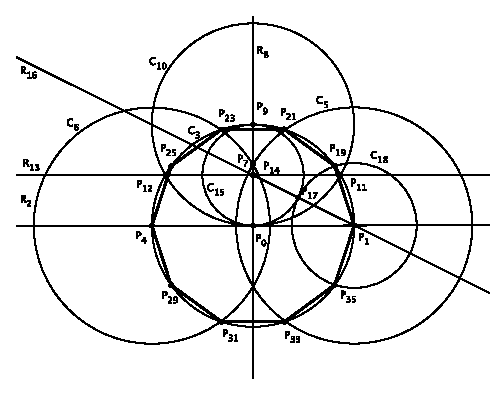
\includegraphics{3_decagon}} 
%\includegraphics{Decagono} 
\caption{Costruzione del decagono}
\end{center}
\end{figure}

Unendo i passaggi appena elencati, si ottiene la costruzione del decagono:
%%%%%%%%%%%%%%%%%%%%%%%%%%%%%%%%%%%%%%% Poly 10
\begin{align*}
\Theta_{10} =  & S_{1} \cup (P_{9}(C_{3}, R_{8}),  C_{10}(P_{9};\overline{P_{9} P_{0}}), P_{11}(C_{3}, C_{10}), \\
&P_{12}(C_{3}, C_{10}), R_{13}(P_{11}, P_{12}), P_{14}(R_{8}, R_{13})), C_{15}(P_{14};\overline{P_{14} P_{0}}) \\
& R_{16}(P_{1}, P_{14}), P_{17}(C_{15}, R_{16}), C_{18}(P_{1};\overline{P_{1} P_{17}}), P_{19}(C_{3},C_{18}) \\
&C_{20}(P_{19};\overline{P_{19} P_{1}}), P_{21}(C_{3}, C_{20}), C_{22}(P_{21};\overline{P_{21} P_{19}}), P_{23}(C_{3}, C_{22}), \\
&C_{24}(P_{23};\overline{P_{23} P_{21}}), P_{25}(C_{3}, C_{24}), C_{26}(P_{25};\overline{P_{25} P_{23}}), P_{27}(C_{3}, C_{26}), \\
&C_{28}(P_{27};\overline{P_{27} P_{25}}), P_{29}(C_{3}, C_{28}), C_{30}(P_{29};\overline{P_{29} P_{27}}), P_{31}(C_{3}, C_{30}), \\
&C_{32}(P_{31};\overline{P_{31} P_{29}}), P_{33}(C_{3}, C_{32}), C_{34}(P_{33};\overline{P_{33} P_{31}}), P_{35}(C_{3}, C_{34}))
\end{align*}

\noindent
Si ha che $\delta_{10}^{0} := P_{1} $ e $\delta_{10}^{k+1} := P_{19 + 2k}$ per $k = 0 \dots 8$.
\\
Per costruire il pentagono $\Theta_{5}$ è sufficiente considerare solo i vertici del tipo $\delta_{10}^{2k}$ per $k = 0 \dots 4 $ del decagono appena costruito.

%%%%%%%%%%%%%%%%%%%%%%%%%%%%%%% EPTADECAGONO
\subsection{Costruzione dell'eptadecagono}

Si propone la costruzione dell'eptadecagono regolare inscritto nella circonferenza di centro $P_{0}$ e raggio $P_{0} P_{1}$, in modo che $P_{1}$ equivalga al primo vertice $\delta_{17}^{0}$:

\begin{enumerate}
% 1
\item Si tracci la costruzione $S_1$ di \ref{perp}, per ottenere le rette perpendicolari $R_{2}(P_{0}, P_{1})$ ed $R_{8}(P_{0}, P_{7})$.
%2
\item Si evidenzi il punto $P_{9}(C_{3}, R_{8})$. Si costruisca il punto $P_{x_1}$ sul segmento $P_{0}P_{9}$, tale che $P_{0}P_{x_1} = \frac{1}{4}P_{0}P_{9}$, con il seguente procedimento: 
\begin{align*}
& P_{9}(C_{3},R_{8}), C_{10}(P_{9};\overline{P_{9} P_{0}}), P_{11}(C_{3}, C_{10}), P_{12}(C_{3}, C_{10}), R_{13}(P_{11}, P_{12}), \\
& P_{14}(R_{8}, R_{13}), C_{15}(P_{14};\overline{P_{14} P_{0}}), C_{16}(P_{0};\overline{P_{14} P_{0}}), P_{17}(C_{15}, C{16}), \\
& P_{18}(C_{15}, C{16}), R_{19}(P_{17}, P_{18}), P_{20}(R_{8}, R_{19}) = P_{x_1}
\end{align*}
%3
\item Si suddivida l'angolo $\angle P_{0}P_{20}P_{1}$ in $4$ parti uguali, in modo da ottenere il punto $P_{x_2}$ sul segmento $P_{0}P_{1}$, tale che $\angle P_{0}P_{20}P_{x_2} = \frac{1}{4} \angle P_{0}P_{20}P_{1}$. Si propone il seguente procedimento:
\begin{align*}
& R_{21}(P_{1},P_{20}), C_{22}(P_{20};\overline{P_{20} P_{21}}), P_{23}(R_{8}, C_{22}), C_{24}(P_{23};\overline{P_{20} P_{1}}), \\
& C_{25}(P_{1};\overline{P_{20} P_{1}}), P_{26}(C_{24}, C_{25}), R_{27}(P_{20}, P_{26}), P_{28}(R_{27}, C_{22}), \\
& C_{29}(P_{28};\overline{P_{28} P_{23}}), C_{30}(P_{23}; \overline{P_{28} P_{23}}), P_{31}(C_{29}, C_{30}), R_{32}(P_{20} P_{31}), \\
& P_{33} (R_{2}, R_{32}) =  P_{x_2}
\end{align*}
%4
\item Si trovi il punto $P_{x_3}$ su $R_2$, tale che $\angle P_{33}P_{20}P_{x_3} = \pi/4$. Si procede nel seguente modo:
\begin{align*}
& P_{34}(C_{22},R_{32}), P_{35}(C_{22},R_{32}), C_{36}(P_{35};\overline{P_{34} P_{35}}), C_{37}(P_{34};\overline{P_{34} P_{35}}), \\
& P_{38}(C_{36},C_{37}), R_{39}(P_{38}, P_{20}), P_{40}(R_{39}, C_{22}), C_{41}(P_{40};\overline{P_{40} P_{35}}), \\
&  C_{42}(P_{35};\overline{P_{40} P_{35}}), P_{43}(C_{41}, C_{42}), R_{44}(P_{43}, P_{20}), P_{45}(R_{44}, R_{2}) = P_{x_3}
\end{align*}
%5
\item Si costruisca la circonferenza avente per diametro $P_{1}P_{45}$, con il seguente procedimento:
\begin{align*}
& C_{46}(P_{45};\overline{P_{45} P_{1}}), C_{47}(P_{1};\overline{P_{45} P_{1}}), P_{48}(C_{46}, C_{47}), P_{49}(C_{46}, C_{47}), \\
& R_{50}(P_{48}, P_{49}), P_{51}(R_{50}, R_{2}), C_{52}(P_{51};\overline{P_{51} P_{1}})
\end{align*}
%6
\item Si evidenzi il punto $P_{53}(C_{52}, R_{8})$che il cerchio $C_{52}$ appena costruito taglia sul segmento $P_{0}P_{9}$ della retta $R_{8}$.
%7
\item Si costruisca la circonferenza $C_{54}(P_{33};\overline{P_{33} P_{53}})$ avente per centro $P_{33}$ e per raggio $P_{33}P_{53}$, si evidenzi il punto che essa taglia sul segmento $P_{0}P_{1}$ con $P_{55}(C_{54}, R_{2})$.
 %8
\item La perpendicolare ad $R_{2}$ passante per l'ultimo punto costruito $P_{55}$ interseca la circonferenza $C_{3}$ nel terzo vertice $\delta_{17}^{3}$ dell'eptadecagono. Si procede alla costruzione di tale vertice nel seguente modo: 
\begin{align*}
& C_{56}(P_{55};\overline{P_{55} P_{33}}), P_{57}(R_{2},C_{56}), C_{58}(P_{33};\overline{P_{37} P_{33}}), C_{59}(P_{37};\overline{P_{37} P_{33}}), \\ 
& P_{60}(C_{58},C_{59}), R_{61}(P_{55},P_{60}), P_{62}(R_{61}, C_{3}) = \delta_{17}^{3}
\end{align*}
%9
\item Il vertice appena costruito consentirà di ricavare tutti gli altri, con la seguente successione di circonferenze e di punti:
\begin{align*}
&C_{63}(P_{62};\overline{P_{62} P_{1}}), P_{64}(C_{3}, C_{63}) = \delta_{17}^{6}, C_{65}(P_{64};\overline{P_{64} P_{62}}), P_{66}(C_{3}, C_{65}) = \delta_{17}^{9},\\
&C_{67}(P_{66};\overline{P_{66} P_{64}}), P_{68}(C_{3}, C_{67})= \delta_{17}^{12}, C_{69}(P_{68};\overline{P_{68} P_{66}}), P_{70}(C_{3}, C_{69})= \delta_{17}^{15},\\
&C_{71}(P_{70};\overline{P_{70} P_{68}}), P_{72}(C_{3}, C_{71}) = \delta_{17}^{1}, C_{73}(P_{72};\overline{P_{72} P_{70}}), P_{74}(C_{3}, C_{73})= \delta_{17}^{4},\\
&C_{75}(P_{74};\overline{P_{74} P_{72}}), P_{76}(C_{3}, C_{75})= \delta_{17}^{7}, C_{77}(P_{76};\overline{P_{76} P_{74}}), P_{78}(C_{3}, C_{77})= \delta_{17}^{10},\\
&C_{79}(P_{78};\overline{P_{78} P_{76}}), P_{80}(C_{3}, C_{79}) = \delta_{17}^{13}, C_{81}(P_{80};\overline{P_{80} P_{78}}), P_{82}(C_{3}, C_{81}) = \delta_{17}^{16},\\
&C_{83}(P_{82};\overline{P_{82} P_{80}}), P_{84}(C_{3}, C_{83})= \delta_{17}^{2}, C_{85}(P_{84};\overline{P_{84} P_{82}}), P_{86}(C_{3}, C_{85})= \delta_{17}^{5},\\
&C_{87}(P_{86};\overline{P_{86} P_{84}}), P_{88}(C_{3}, C_{87})= \delta_{17}^{8}, C_{89}(P_{88};\overline{P_{88} P_{86}}), P_{90}(C_{3}, C_{89})= \delta_{17}^{11},\\
&C_{91}(P_{90};\overline{P_{90} P_{88}}), P_{92}(C_{3}, C_{91}) = \delta_{17}^{14} 
\end{align*}
\end{enumerate}

Unendo i passaggi appena elencati, si ottiene la costruzione dell'eptadecagono:
%%%%%%%%%%%%%%%%%%%%%%%%%%%%%%%%%%%%%%% Poly 17
\begin{align*}
\Theta_{17} =  & S_{1} \cup (P_{9}(C_{3}, R_{8}),  C_{10}(P_{9};\overline{P_{9} P_{0}}), P_{11}(C_{3}, C_{10}), P_{12}(C_{3}, C_{10}), \\
& R_{13}(P_{11}, P_{12}), P_{14}(R_{8}, R_{13})), C_{15}(P_{14};\overline{P_{14} P_{0}}), C_{16}(P_{0}; \overline{P_{0} P_{14}}), \\ 
& P_{17}(C_{15}, C_{16}), P_{18}(C_{15}, C_{16}) R_{19}(P_{17}, P_{18}), P_{20}(R_{8}, R_{19}), R_{21}(P_{1},P_{20}), \\ 
& C_{22}(P_{20};\overline{P_{20} P_{21}}), P_{23}(R_{8}, C_{22}), C_{24}(P_{23};\overline{P_{20} P_{1}}), C_{25}(P_{1};\overline{P_{20} P_{1}}),\\ 
& P_{26}(C_{24}, C_{25}), R_{27}(P_{20}, P_{26}), P_{28}(R_{27}, C_{22}), C_{29}(P_{28};\overline{P_{28} P_{23}}), \\ 
& C_{30}(P_{23}; \overline{P_{28} P_{23}}), P_{31}(C_{29}, C_{30}), R_{32}(P_{20} P_{31}), P_{33} (R_{2}, R_{32}), P_{34}(C_{22},R_{32}), \\ 
& P_{35}(C_{22},R_{32}), C_{36}(P_{35};\overline{P_{34} P_{35}}), C_{37}(P_{34};\overline{P_{34} P_{35}}), P_{38}(C_{36},C_{37}), \\
& R_{39}(P_{38}, P_{20}), P_{40}(R_{39}, C_{22}), C_{41}(P_{40};\overline{P_{40} P_{35}}), C_{42}(P_{35};\overline{P_{40} P_{35}}), \\
& P_{43}(C_{41}, C_{42}), R_{44}(P_{43}, P_{20}), P_{45}(R_{44}, R_{2}), C_{46}(P_{45};\overline{P_{45} P_{1}}), \\
& C_{47}(P_{1};\overline{P_{45} P_{1}}), P_{48}(C_{46}, C_{47}), P_{49}(C_{46}, C_{47}), R_{50}(P_{48}, P_{49}), P_{51}(R_{50}, R_{2}), \\
& C_{52}(P_{51};\overline{P_{51} P_{1}}), P_{53}(C_{52}, R_{8}), C_{54}(P_{33};\overline{P_{33} P_{53}}), P_{55}(C_{54}, R_{2}), \\
& C_{56}(P_{55};\overline{P_{55} P_{33}}), P_{57}(R_{2},C_{56}), C_{58}(P_{33};\overline{P_{37} P_{33}}), \\
& C_{59}(P_{37};\overline{P_{37} P_{33}}), P_{60}(C_{58},C_{59}), R_{61}(P_{55},P_{60}), P_{62}(R_{61}, C_{3}) \\
&C_{63}(P_{62};\overline{P_{62} P_{1}}), P_{64}(C_{3}, C_{63}), C_{65}(P_{64};\overline{P_{64} P_{62}}), P_{66}(C_{3}, C_{65}),\\
&C_{67}(P_{66};\overline{P_{66} P_{64}}), P_{68}(C_{3}, C_{67}), C_{69}(P_{68};\overline{P_{68} P_{66}}), P_{70}(C_{3}, C_{69}),\\
&C_{71}(P_{70};\overline{P_{70} P_{68}}), P_{72}(C_{3}, C_{71}), C_{73}(P_{72};\overline{P_{72} P_{70}}), P_{74}(C_{3}, C_{73}),\\
&C_{75}(P_{74};\overline{P_{74} P_{72}}), P_{76}(C_{3}, C_{75}), C_{77}(P_{76};\overline{P_{76} P_{74}}), P_{78}(C_{3}, C_{77}),\\
&C_{79}(P_{78};\overline{P_{78} P_{76}}), P_{80}(C_{3}, C_{79}), C_{81}(P_{80};\overline{P_{80} P_{78}}), P_{82}(C_{3}, C_{81}),\\
&C_{83}(P_{82};\overline{P_{82} P_{80}}), P_{84}(C_{3}, C_{83}), C_{85}(P_{84};\overline{P_{84} P_{82}}), P_{86}(C_{3}, C_{85}),\\
&C_{87}(P_{86};\overline{P_{86} P_{84}}), P_{88}(C_{3}, C_{87}), C_{89}(P_{88};\overline{P_{88} P_{86}}), P_{90}(C_{3}, C_{89}),\\
&C_{91}(P_{90};\overline{P_{90} P_{88}}), P_{92}(C_{3}, C_{91}) ) 
\end{align*}

\noindent
Si ha che $\delta_{17}^{0} := P_{1}$, $\delta_{17}^{3} := P_{62}$ e $\delta_{17}^{4k+1} := P_{64 + 2k}$ per $k = 0 \dots 15$.

%%%%%%%% IMMAGINE COSTRUZIONE EPTADECAGONO %
\begin{figure}[!h]
%centrare
\begin{center}
\resizebox{12.7 cm}{9.5 cm}{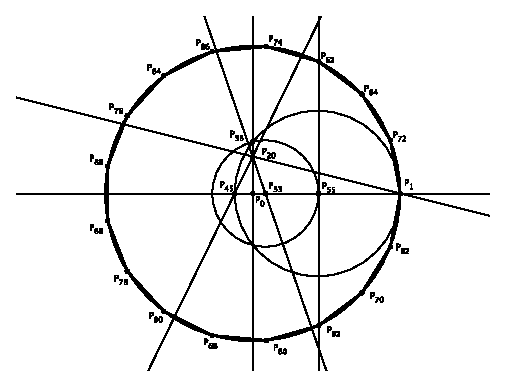
\includegraphics{3_eptadecagon}} 
%\includegraphics{Es1perpendicolare} 
\caption{Costruzione dell'eptadecagono}
\end{center}
\end{figure}


%FINE CAP 3

% LABELS:
%
%\label{potcompl}  prop potenze n-esime di un numero complesso
%\label{osservazionedue}   seconda osservazione par 3.2
%\label{teoremaprimo} Sulla costruibilità per phi
%\label{lemmaprimo}
%\label{lemmasecondo}
%\label{teoremaciclotomia}




%%%%%%%%%%%%%%%%%%%%%%%%%%%%%%%%%%%%%%%%%%%%%%%%%%%%%%%%%%%%%%%%%%%%%%%%%%%%%%%%%%%%%%%%%%%%%%%%%%%%%%%%%%%%%%%%%%%%%%%%%%%%%%%%%%%%%%%%%%%%%%%%%%%%%%%%%%%%%%%%%%%%%%%%







\chapter{Tre problemi impossibili}

In quest'ultimo capitolo si affronta il tema centrale di questa tesi. Si hanno infatti le basi per dimostrare rigorosamente che, con il solo uso di riga e compasso, non è possibile trovare il lato di un cubo avente volume doppio di un cubo dato, suddividere un angolo dato in tre angoli uguali e costruire un quadrato di area uguale a quella di un cerchio dato.


%%%%%%%%%%%%%%%%%%%%% SEZIONE
\section{Duplicazione del cubo}
Dato un cubo di lato $l$ e di volume $l^3 = v$, per costruirne uno di volume doppio di lato $l'$, si deve tracciare un segmento che soddisfi la seguente equazione

\begin{align*}
l'^3 = 2v
\end{align*}

Quindi $l' = \sqrt[3]{2v}$. Possiamo sempre porre $l = 1$ utilizzando l'unità di misura $l$ come il segmento di lunghezza $P_0 P_1$, da cui si ha $v = 1$, e quindi 

\begin{align*}
l' = \sqrt[3]{2}
\end{align*}

Questo implica che $l'$ soddisfa il polinomio $x^3 - 2$ irriducibile su $\mathbb{Q}$; per il corollario \ref{corollb} $l'$ non è costruibile.


%%%%%%%%%%%%%%%%%%%%% SEZIONE
\section{Trisezione dell'angolo}
Non tutti gli angoli dati possono essere sempre trisecati: sia ad esempio\footnote{Da \cite{cattaneo} pag. $347$. } $\alpha = 3\theta = \pi / 3$, allora costruire l'angolo di $\theta = \pi / 9$ equivale a costruire $cos(\pi / 9)$. 
Dalle note relazioni trigonometriche si ottiene
\begin{align*}
cos(3\theta) = 4 cos^3(\theta) - 3 cos(\theta)
\end{align*}

Da cui per $3\theta = \pi / 3$, si ha che
\begin{align*}
1/2 = 4 cos^3(\pi / 9) - 3 cos(\pi / 9)
\end{align*}

Quindi $cos(\pi / 9)$ soddisfa il polinomio 
\begin{align*}
8x^3 - 6x - 1 = 0 
\end{align*}

\noindent
irriducibile su $\mathbb{Q}$, di grado $3$. Quindi per il corollario \ref{corolla} $cos(\pi / 9)$ non è costruibile.
\\\\
Alcuni angoli possono essere trisecati; ad esempio quello di $(3/4)\pi$ formato dalle semirette $r_1$ ed $r_2$. Con il procedimento \ref{perp} e \ref{bisett} è possibile costruire prima una retta $s_1$ perpendicolare a $r_1$ e poi la bisettrice di $r_1$ ed $s_1$, indicata con $s_2$. In questo modo l'angolo fra $r_1$ ed $r_2$ è trisecato dalle rette $s_1$ ed $s_2$.

%%%%%%%%%%%%%%%%%%%%%%%%%%%%
%%%%%%%%%%%%%%%%%%%%%%%%%% TRASCENDENZA DI e
\section{Trascendenza di $e$ e di $\pi$} \label{trascendenzapi}

La necessità di determinare se un dato numero sia algebrico, cioè radice di un polinomio a coefficienti interi, o viceversa trascendente, si presentò per la prima volta a metà del 1800 da Joseph Liouville (Saint Omer, 1809 - Parigi, 1882). Egli infatti dimostrò l'esistenza dei numeri trascendenti, affermando che ogni numero della forma
\begin{align*}
\frac{a_1}{10} + \frac{a_1}{10^{2!}} + \frac{a_1}{10^{3!}} + \cdots  
\end{align*}
\noindent
con ${a_i}$ numeri interi arbitrari, compresi fra $0$ e $9$, è trascendente. 
\\
A questo punto si presenta il secondo protagonista della storia dei numeri trascendenti, Charles Hermite (Dieuze, 1822 - Parigi, 1901), il quale, tentando di dimostrare la trascendenza di $\pi$, giunse nel 1873 a dimostrare la trascendenza del numero di Nepero.
Dopo questo successo scrisse in una lettera indirizzata al collega tedesco Carl Wilhelm Brochardt (Berino, 1817 - Ruedesdorf 1880) le seguenti parole:\footnote{Da \cite{kline} pag. $1146$. }

\begin{center}
\emph{ \lq\lq Non oso tentare di dimostrare la trascendenza di $\pi$. Se altri ci riusciranno, nessuno sarà più felice di me per il loro successo, ma credimi, caro amico, ciò non mancherà di costare loro qualche sforzo.\rq\rq }
\end{center}

L'artefice della felicità di Hermite, fu Carl Louis Ferdinand von Lindemann (Hannover, 1852 - Gottinga, 1939), che nel 1882 scoprì la trascendenza di $\pi$. Egli arrivò a dimostrare che se $x_1, x_2, \dots x_n$ sono numeri algebrici distinti, reali o complessi, e se $p_1, p_2, \dots p_n$ sono numeri algebrici non tutti nulli, allora la somma
\begin{align*}
p_1 e^{x_1} + p_2 e^{x_2} + \cdots + p_n e^{x_n}  
\end{align*}
\noindent
è sempre diversa da zero. Da tale fatto, per $n = 2$, $p_1 = p_2 = 1$ e $x_2 = 0$ si ha 
\begin{align*}
e^{x_1} + 1 \neq 0  
\end{align*}
\noindent
per ogni $x_1$ algebrico. Ma per la formula di Eulero $e^{i\pi} + 1 = 0$ si ha che $i\pi$ deve essere trascendente, e dato che $i$ è algebrico, si ha che $\pi$ deve essere trascendente\footnote{Per la dimostrazione completa della trascendenza di $e$ e $\pi$, vedere ad esempio \cite{Stewart} Teorema $6.4$ di pag. $72$, oppure \cite{Baker} pag. $6$. }.
Tale dimostrazione di teoria dei numeri, assieme alla teoria dei campi applicata alle costruzioni con riga e compasso, ha risolto definitivamente il problema della quadratura del cerchio che aveva tenuto occupati i matematici di ogni epoca.

%%%%%%%%%%%%%%%%%%%%%%%%%
%%%%%%%%%%%%%%%%%%%%%% SEZIONE
\section{Quadratura del cerchio} \label{quadratura}
Preso un cerchio di raggio $r$ e area $a = \pi r^2$, si vuole costruire un quadrato della stessa area. Possiamo sempre porre $r = 1$ utilizzando l'unità di misura $r$ come il segmento di lunghezza $P_0 P_1$ da cui $a = \pi$. Per risolvere il problema, si deve allora costruire un segmento di lunghezza $\sqrt{\pi}$ ma dato che, come visto in \ref{trascendenzapi}, $\pi$ è trascendente, si ha che non appartiene a nessun ampliamento di $\mathbb{Q}$ avente grado una potenza di due. Non è quindi costruibile.

%%%%%%%%%%%%%%%%%%%%%% SEZIONE
\section{Rettificazione della circonferenza}
In analogia con il problema \ref{quadratura} sulla quadratura del cerchio, si può chiedere di risolvere con riga e compasso il seguente problema: data una circonferenza di raggio $r$ e lunghezza $h = 2\pi r$ si richiede la costruzione di un segmento di lunghezza pari ad $h$. Possiamo sempre porre $r = 1$ utilizzando l'unità di misura $r$ come il segmento di lunghezza $P_0 P_1$, da cui si ha $h = 2\pi$. Ma anche in questo caso, come nel precedente, il segmento di lunghezza $2\pi$ non è costruibile, in virtù della trascendenza di $\pi$.














%\input{5cap.tex}

%questo va messo nell'appendice!

\chapter*{Appendice}



I lettori di questa tesi si saranno chiesti come mai così tanti matematici hanno trascorso molto tempo a cercare una soluzione dei tre problemi classici, usando esclusivamente riga e compasso, nonostante avessero a disposizione una soluzione trovata con mezzi più moderni. In queste poche righe, vorrei provare a spiegare che la loro non è stata solo la ricerca della soddisfazione personale, ma è conseguenza di motivazioni filosofiche e inaspettatamente pratiche. \\

Come è noto, negli Elementi di Euclide, la riga e il compasso sono alla base di un sistema assiomatico, che una volta finito nelle mani dei matematici successivi è stato ammirato per la sua forma, eleganza e per la sua completezza. \\
In verità le lacune degli Elementi sono molteplici; per esempio nella costruzione del triangolo equilatero si usa una proprietà che non viene mai ne dimostrata ne espressa chiaramente, cioè che due circonferenze, con centro sui diversi estremi di un segmento e aventi per raggio il segmento stesso, abbiano intersezione non vuota \cite{Shea}. \\
Basandosi sull'osservazione di questa ed altre lacune, lo studioso Lucio Russo \cite{Russo}, sostiene che gli Elementi non sono altro che una sorta di manuale di istruzioni per utilizzare il più potente calcolatore dell' epoca: la riga e il compasso.
L'idea che ogni figura geometrica pensabile sia costruibile e quindi misurabile direttamente con questi due oggetti ci porterebbe a credere che i greci avessero sviluppato un sistema completo, elegante e soprattutto definitivo.\\

A questo punto l'impossibilità di risolvere i tre problemi classici, arrivata per via algebrica, ha dimostrato la necessità di affrontare nuovi orizzonti. Ha dato quindi un contributo fondamentale a rendere, già nella seconda metà dell'ottocento, non del tutto soddisfacente la visione della geometria fornita dall'opera di Euclide. 





%%%%%%%%%%%%% BIBLIOGRAFIA  %%%%%%%%%%%%%%%%%%%%%%%%%%%
%%%%%%%%%%%%%%%%%%%%%%%%%%%%%%%%%%%%%%%%%%%%%%%%
\newpage

\begin{thebibliography}{21}

\bibitem{Artin}
Michael Artin, \emph{Algebra}, Prentice Hall of India, New Delhi 2007 

\bibitem{Baker}
Alan Baker, \emph{Transcendental Number theory}, Cambridge univesity press 1990, prima ed. 1975.

\bibitem{Dante}
Dante Alighieri, \emph{La Divina Commedia}, Einaudi 1954.

\bibitem{Boyer}
Carl B. Boyer, \emph{Storia della matematica}, Mondadori 2005, prima ed. 1976.

\bibitem{kline}
Morris Kline \emph{Storia del pensiero matematico, dal settecento ad oggi}, volume secondo, Einaudi editore 1991.

\bibitem{Kosh}
Thomas Koshy, \emph{Elementary Number Theory with applications}, Accademic Press, Elzevier, 2007.

\bibitem{Livio}
Mario Livio, \emph{L'equazione impossibile}, BUR 2007, prima ed. 2006.

\bibitem{Shea}
Donald O'Shea, \emph{La congettura di Poincarè}, BUR, Milano 2007.

\bibitem{cattaneo}
Giulia Maria Piacentini Cattaneo, \emph{Algebra, un approccio algoritmico}, Zanichelli 2007, prima ed. 1996.

\bibitem{Plato}
Platone, \emph{Dialoghi}.

\bibitem{Procesi}
Claudio Procesi, \emph{Elementi di teoria di Galois}, Zanichelli 2008, prima ed. 1977.

\bibitem{Rogg}
Margherita Roggero, \emph{Appunti ed esercizi di Matematica Discreta}, Quaderni didattici dell'Università di Torino, 2005.

\bibitem{Russo}
Lucio Russo, \emph{La rivoluzione dimenticata: il pensiero scientifico greco e la scienza moderna}, Feltrinelli Milano 1997.

\bibitem{Shanks} 
Daniel Shanks \emph{Solved and unsolved problems in Number Theory }, AMS 1993, prima ed. 1962

\bibitem{Stewart}
Ian Stewart, \emph{Galois Theory}, Chapman and Hall 1973, prima ed. 2006.

\bibitem{sitowolfram}
Dal Web: sito della Wolfram Research, pagina sulla costruzione dell'eptadecagono:  \begin{verbatim} http://mathworld.wolfram.com/Heptadecagon.html \end{verbatim}

\bibitem{sitoroi}
Dal Web: sito del prof. Lorenzo Roi, pagina sulla costruzione del decagono e dell'eptadecagono: \begin{verbatim} http://www.lorenzoroi.net/geometria/Poligoni.html \end{verbatim}

\bibitem{sito3}
Da Wikipedia, sulla trisezione dell'angolo: \begin{verbatim} http://it.wikipedia.org/wiki/Trisezione_dell'angolo \end{verbatim}

\bibitem{sito2}
Da Wikipedia, sul problema di Delo: \begin{verbatim} http://it.wikipedia.org/wiki/Problema_di_Delo \end{verbatim}

\bibitem{sito2}
Da Wikipedia, sulla quadratura del cerchio: \begin{verbatim} http://it.wikipedia.org/wiki/Quadratura_del_cerchio \end{verbatim}

\bibitem{sito4}
Da Wikipedia, sulla costruzione dell'eptadecagono: \begin{verbatim} http://it.wikipedia.org/wiki/Eptadecagono \end{verbatim}

\end{thebibliography}

\end{document}





















